\documentclass[11pt,a4paper]{article}

\usepackage[utf8]{inputenc}
\usepackage[vietnamese,english]{babel}
\usepackage[T5,T1]{fontenc}
\usepackage{lmodern}
\usepackage[margin=2.2cm]{geometry}
\usepackage{amsmath,amsfonts,amssymb,amsthm}
\usepackage{booktabs}
\usepackage{multirow}
\usepackage{graphicx}
\usepackage{hyperref}
\usepackage{microtype}
\usepackage{xcolor}
\usepackage{cite}
\usepackage{titlesec}
\usepackage{caption}

\hypersetup{
    colorlinks=true,
    linkcolor=blue!80!black,
    citecolor=red!70!black,
    urlcolor=blue!70!black,
    pdfauthor={Phạm Khánh Duy},
    pdftitle={Nghiên cứu các Kỹ thuật Mã hóa SAT cho Bài toán N-Queens}
}
}

\newtheorem{definition}{Định nghĩa}
\newtheorem{theorem}{Định lý}
\newtheorem{lemma}{Bổ đề}
\newtheorem{proposition}{Mệnh đề}

\title{\Large \textbf{Nghiên cứu các Kỹ thuật Mã hóa SAT cho Bài toán N-Queens và So sánh Thực nghiệm với Quy hoạch Tuyến tính Nguyên (ILP) và Lập trình Ràng buộc (CP)}}

\author{
    \textbf{Phạm Khánh Duy}$^{1}$ \quad \textbf{TS. Tô Văn Khánh}$^{1,*}$ \\[0.5em]
    $^{1}$Khoa Công nghệ Thông tin, Trường Đại học Công nghệ, ĐHQGHN, Hà Nội, Việt Nam \\
    \texttt{\{24021452, khanhtv\}@vnu.edu.vn}
}

\date{Tháng 10 năm 2026}

\let\printorcid\relax
\begin{document}
\selectlanguage{vietnamese}
\maketitle

\begin{abstract}
Bài toán $N$-Queens là bài toán kinh điển trong khoa học máy tính và tối ưu tổ hợp rời rạc, yêu cầu sắp xếp $N$ quân hậu trên bàn cờ $N \times N$ không tấn công lẫn nhau. Khi kích thước $N$ gia tăng, không gian tìm kiếm bùng nổ theo giai thừa $\mathcal{O}(N!)$, tạo ra thách thức lớn cho các bộ giải chính xác. Bài báo này nghiên cứu tiếp cận giải chính xác $N$-Queens bằng SAT Solving qua thư viện PySAT. Trọng tâm nghiên cứu là phân tích lý thuyết và đánh giá thực nghiệm 5 kỹ thuật mã hóa At-Most-One (AMO): Pairwise, Sequential Counter, Commander Variable, Binary (Prestwich, 2009; Frisch \& Giannaros, 2010) và Product Encoding. Kết quả đo đạc chuẩn hóa qua các tiến trình độc lập (\texttt{subprocess}) cho thấy Pairwise bùng nổ $\mathcal{O}(N^3)$ mệnh đề, tiêu tốn khoảng 7.7 GB RAM đỉnh tại $N=256$ ($7{,}679.4$ MB) và dừng do ngoại lệ \texttt{MemoryError} khi khởi tạo $207.8$ triệu mệnh đề tại $N=500$. Ngược lại, Sequential, Product và Commander duy trì bậc $\mathcal{O}(N^2)$ mệnh đề. Về hiệu năng giải bằng CaDiCaL 1.9.5, Commander Variable đạt tốc độ nhanh nhất trên dải $N \in [16, 128]$ (chỉ mất $0.76$s ở $N=128$, nhanh hơn Sequential khoảng 33 lần). Ở quy mô cực đại $N \ge 256$, Commander mở rộng thành công ổn định 3/3 lần lên tới $N=500$ ($32.11$s) và $N=1000$ ($100.92$s); Product đạt 3/3 lần thành công ở $N=500$ ($32.26$s) và đạt tỷ lệ thành công 2/3 lần ở $N=1000$ ($200.36$s; 1 lần chạm giới hạn thời gian 300.0s). Thực nghiệm 3 lần chạy lặp độc lập quan sát thấy tính tất định của CaDiCaL với số lượng xung đột và quyết định đồng nhất $100\%$ trên cùng công thức CNF; sự biến thiên thời gian giải ở quy mô lớn được phân tích dưới các giả thuyết về điều tiết xung nhịp phần cứng và quản lý bộ nhớ đệm hệ điều hành. So sánh đối chứng đơn luồng (Time Limit 300.0s) với CP-SAT (Google OR-Tools), Gurobi 13.0 và SCIP 9.0 cho thấy SAT Solving vượt trội về tính mở rộng ở $N \ge 256$, trong khi Gurobi dừng ở $N \ge 64$ do giới hạn kích thước license đi kèm gói pip (tối đa 2.000 biến).
\end{abstract}

\noindent\textbf{Từ khóa:} $N$-Queens, SAT Solving, PySAT, CaDiCaL, At-Most-One (AMO), Commander Variable, Product Encoding, Constraint Programming (CP), Integer Linear Programming (ILP), Gurobi.

\vspace{1em}
\hrule
\vspace{1.5em}

\section{Giới thiệu (Introduction)}

\noindent\textbf{1. Bối cảnh lịch sử và Định nghĩa bài toán:}\\
Bài toán $N$-Queens (xếp $N$ quân hậu) được nhà nghiên cứu Max Bezzel khởi xướng vào năm 1848 dưới dạng bài toán 8 quân hậu trên bàn cờ vua tiêu chuẩn, và nhanh chóng thu hút sự chú ý của các nhà toán học lừng danh, tiêu biểu là Carl Friedrich Gauss~\cite{bell2009survey}. Về mặt hình thức, bài toán yêu cầu đặt $N$ quân hậu lên một bàn cờ kích thước $N \times N$ sao cho không có bất kỳ hai quân hậu nào có thể tấn công lẫn nhau. Theo luật cờ vua, điều này đồng nghĩa với việc không có hai quân hậu nào nằm trên cùng một hàng, cùng một cột, hoặc cùng một đường chéo (chính hoặc phụ).

\noindent\textbf{2. Ý nghĩa lý thuyết và Ứng dụng thực tiễn:}\\
Mặc dù có cấu trúc phát biểu trực quan và đơn giản, $N$-Queens là bài toán chuẩn mực (standard benchmark) để kiểm tra năng lực của các thuật toán tìm kiếm tổ hợp, kỹ thuật thỏa mãn ràng buộc (CSP - Constraint Satisfaction Problem), giải thuật heuristic và các bộ giải suy diễn logic~\cite{rossi2006handbook}. Ngoài ý nghĩa lý thuyết, các biến thể của bài toán $N$-Queens xuất hiện trong nhiều ứng dụng công nghiệp thực tiễn quan trọng như: thiết kế bố trí vi mạch tích hợp cỡ lớn (VLSI design), định tuyến thông tin trong mạng truyền thông đa xử lý song song, lập lịch tài nguyên không xung đột, và xây dựng các khối mã kiểm tra sửa lỗi trong mật mã học~\cite{bell2009survey}.

\noindent\textbf{3. Các hướng tiếp cận giải quyết bài toán:}\\
Để giải quyết bài toán $N$-Queens, cộng đồng khoa học đã phát triển nhiều hướng tiếp cận khác nhau:
\begin{enumerate}
    \item \textbf{Tìm kiếm vét cạn và Quay lui (Backtracking):} Là phương pháp cổ điển, tuy nhiên chi phí tính toán tăng giai thừa khiến thuật toán quay lui thuần túy gặp khó khăn lớn khi $N$ tăng.
    \item \textbf{Heuristic và Tìm kiếm cục bộ (Local Search):} Các giải thuật tìm kiếm xung đột tối thiểu (Min-Conflicts) của Minton et al.~\cite{minton1992solving} có thể tìm một nghiệm khả dĩ cho bàn cờ rất lớn trong thời gian ngắn, nhưng không mang tính chất chứng minh chính xác (exact method) và không áp dụng được khi cần chứng minh bài toán vô nghiệm trong các biến thể mở rộng như $N$-Queens có ô cấm ($N$-Queens Completion)~\cite{gent2017complexity}.
    \item \textbf{Quy hoạch Tuyến tính Nguyên (Integer Linear Programming - ILP):} Biểu diễn bài toán thành hệ các phương trình và bất phương trình tuyến tính trên biến nguyên $0-1$~\cite{wolsey2020integer}. Mặc dù các bộ giải thương mại như Gurobi Optimizer~\cite{gurobi} rất mạnh mẽ, bài toán $N$-Queens gây khó khăn lớn cho ILP khi $N$ tăng vì nghiệm nới lỏng tuyến tính (LP relaxation) cho giá trị phân số đồng nhất $x_{i,j} = 1/N$, làm suy giảm hiệu quả của nhánh-cận (Branch-and-Bound).
    \item \textbf{Lập trình Ràng buộc (Constraint Programming - CP):} Mô hình hóa vị trí quân hậu bằng các biến chỉ số cột kèm toán tử toàn cục \texttt{AllDifferent}. Bộ giải hiện đại Google OR-Tools CP-SAT sử dụng cơ chế Lazy Clause Generation đạt hiệu năng rất cao ở các giá trị $N$ nhỏ và trung bình~\cite{ortools}.
    \item \textbf{Mã hóa SAT (SAT Encoding \& Solving):} Chuyển đổi toàn bộ các điều kiện của bài toán thành dạng chuẩn hội (Conjunctive Normal Form - CNF) và sử dụng các bộ giải SAT hiện đại dựa trên kiến trúc CDCL (Conflict-Driven Clause Learning) như CaDiCaL~\cite{biere2024cadical}, Glucose~\cite{audemard2018glucose}. Bộ giải CaDiCaL được tác giả Armin Biere và cộng sự phát triển~\cite{biere2024cadical}, trong đó bản phát hành 1.9.5 được tích hợp sẵn qua cổng giao tiếp C++ của thư viện PySAT~\cite{ignatiev2018pysat}.
\end{enumerate}

\noindent\textbf{4. Thách thức bùng nổ mệnh đề trong tiếp cận SAT:}\\
Trọng tâm của tiếp cận SAT nằm ở việc chuyển đổi các ràng buộc số lượng, cụ thể là ràng buộc \textit{Exactly-One} (Đúng một) và \textit{At-Most-One} (Tối đa một - AMO) thành các mệnh đề logic (clauses). Cách mã hóa cặp trực tiếp (Pairwise) dẫn tới bùng nổ đa thức bậc ba $\mathcal{O}(N^3)$ mệnh đề trên toàn bàn cờ; thực nghiệm của chúng tôi ghi nhận ở $N=256$, Pairwise đòi hỏi tới $27{,}831{,}552$ mệnh đề và tiêu tốn đỉnh điểm khoảng 7.7 GB RAM ($7{,}679.4$ MB, $\approx 7.50$ GiB), và đến $N=500$ mô hình chạm mốc $207{,}834{,}500$ mệnh đề (xấp xỉ $207.8$ triệu), dẫn đến hiện tượng cạn kiệt bộ nhớ (OOM) khi khởi tạo danh sách đối tượng trong Python trên hệ thống 32 GB RAM.

\noindent\textbf{5. Đóng góp khoa học cốt lõi của bài báo:}
\begin{itemize}
    \item Nghiên cứu, cài đặt và phân tích so sánh lý thuyết lẫn thực nghiệm 5 kỹ thuật mã hóa AMO: Pairwise, Sequential Counter~\cite{sinz2005towards}, Commander Variable~\cite{klieber2007efficient}, Binary Encoding~\cite{prestwich2009cnf,frisch2010sat} và Product Encoding~\cite{chen2010product}. Phân định rõ giữa các hàm PySAT CardEnc có sẵn và các thuật toán tự cài đặt độc lập.
    \item Triển khai hoàn chỉnh bộ giải $N$-Queens Solver trên nền tảng PySAT~\cite{ignatiev2018pysat}, tích hợp solver CaDiCaL 1.9.5 và Glucose 4.2.
    \item Thiết lập giao thức đo lường chuẩn hóa: lặp lại đúng 3 lần cho mọi kích thước $N$ được khảo sát của từng kỹ thuật (lên tới $N=1000$ đối với Commander và Product) trong từng tiến trình con độc lập (\texttt{subprocess}) cách ly bộ nhớ hoàn toàn, đo RAM đỉnh thực tế cho từng lần chạy qua \texttt{psutil}, áp dụng cùng Time Limit 300.0 giây, chạy đơn luồng (1 worker / 1 thread) cho tất cả các solver.
    \item Thu thập dữ liệu thực nghiệm vi mô giải thích động lực tìm kiếm CDCL (\textit{search dynamics}): trích xuất thông số nội tại (\texttt{accum\_stats()}) và tính mã băm SHA-256 của từng công thức CNF qua 3 lần chạy lặp. Kết quả thực nghiệm 3 lần chạy lặp độc lập quan sát thấy tính tất định của CaDiCaL trên cùng một CNF với số lượng xung đột và quyết định hoàn toàn đồng nhất ($3/3$ lần trùng khớp), đồng thời chỉ ra sự suy thoái hiệu năng của Sequential Counter ở $N=128$ ($24.85$s, chậm hơn Commander 33 lần) bị dẫn dắt bởi sự tăng vọt $68\times$ số xung đột ($62{,}360$ so với $916$) và $26\times$ số quyết định ($107{,}733$ so với $4{,}159$), kéo theo $42.89$ triệu lượt lan truyền đơn vị. Phân tích thực nghiệm cũng làm rõ mối quan hệ phi tuyến: số lượng biến phụ không quyết định trực tiếp số xung đột (Commander có $33{,}290$ biến phụ, nhiều hơn $2.4\times$ so với Product, nhưng lại có số xung đột thấp nhất chỉ $916$).
    \item So sánh đối chứng toàn diện giữa SAT Solving với Google OR-Tools CP-SAT, Gurobi Optimizer 13.0 và SCIP 9.0 (ILP MIP) trên dải kích thước bàn cờ từ $N = 8$ đến $N = 1000$.
    \item Kết quả thực nghiệm cho thấy CaDiCaL 1.9.5 kết hợp Commander Variable giải quyết thành công 3/3 lần bàn cờ kích thước cực lớn $N = 500$ ($32.11$s) và $N = 1000$ ($1{,}000{,}000$ ô cờ; $100.92$s); kết hợp Product Encoding đạt 3/3 lần thành công ở $N = 500$ ($32.26$s) và đạt tỷ lệ giải thành công 2/3 lần ở $N = 1000$ ($200.36$s; 1 lần chạm trần thời gian 300.0s do chi phí lan truyền trên gần 12 triệu mệnh đề), trong khi CP-SAT và SCIP đều dừng do hết thời gian (timeout) ở $N \ge 256$, còn Gurobi dừng ở $N \ge 64$ do giới hạn kích thước license đi kèm gói pip (2.000 biến).
\end{itemize}

---

\section{Cơ sở lý thuyết và Mô hình hóa (Background \& Formulations)}

\subsection{Phát biểu bài toán N-Queens}
\begin{tcolorbox}[
    colback=boxbg, colframe=boxborder, arc=2mm, boxrule=0.75pt,
    left=10pt, right=10pt, top=7pt, bottom=7pt,
    title=\textbf{\color{primaryblue}Định nghĩa 1 (Bài toán $N$-Queens tiêu chuẩn)},
    coltitle=primaryblue
]
Cho bàn cờ vuông kích thước $N \times N$, tập tọa độ các ô cờ là $\mathcal{H}_N = \{(r, c) \mid 0 \le r, c < N\}$, trong đó $r$ là chỉ số hàng và $c$ là chỉ số cột. Bài toán yêu cầu đặt $N$ quân hậu vào tập vị trí $\mathcal{Q} \subset \mathcal{H}_N$ thỏa mãn:
\begin{align}
    &|\mathcal{Q}| = N, \\
    &\forall (r_1, c_1), (r_2, c_2) \in \mathcal{Q}, \; (r_1, c_1) \neq (r_2, c_2) \implies \nonumber\\
    &\quad r_1 \neq r_2 \quad \land \quad c_1 \neq c_2 \quad \land \quad |r_1 - r_2| \neq |c_1 - c_2|.
\end{align}
\end{tcolorbox}

\subsection{Các nghiên cứu liên quan (Related Work)}

\noindent\textbf{Tiến trình nghiên cứu và Kết quả giải tích:}\\
Nghiên cứu về $N$-Queens đã trải qua hơn 170 năm với nhiều bước tiến lý thuyết và thực nghiệm. Bell và Stevens~\cite{bell2009survey} đã tổng hợp toàn diện các kết quả giải tích, chỉ ra rằng với mọi $N \ge 4$, luôn tồn tại ít nhất một nghiệm hợp lệ, và có thể xây dựng trực tiếp nghiệm bằng các công thức tường minh dựa trên số học modular. Về phương diện giải thuật heuristic, Minton et al.~\cite{minton1992solving} đề xuất thuật toán Min-Conflicts, có thể tìm ra một nghiệm cho $N$ rất lớn trong thời gian ngắn.

\noindent\textbf{Giới hạn của Heuristic và Nhu cầu về Bộ giải chính xác:}\\
Tuy nhiên, các thuật toán heuristic và công thức giải tích chỉ giải quyết bài toán đặt hậu tiêu chuẩn mà không thể khái quát hóa cho các bài toán mở rộng như đếm số lượng nghiệm (\#SAT / Model Counting), hoặc bài toán $N$-Queens có chướng ngại vật ($N$-Queens Completion) vốn đã được Gent et al.~\cite{gent2017complexity} chứng minh là NP-đầy đủ. Do đó, việc nghiên cứu $N$-Queens dưới góc độ các hệ giải quyết ràng buộc chính xác tổng quát (General Exact Solvers) như SAT, CP và ILP giữ vai trò học thuật cốt lõi~\cite{rossi2006handbook,biere2021handbook}. 

\noindent\textbf{Các nghiên cứu nền tảng về kỹ thuật mã hóa AMO trong SAT:}\\
Trong lĩnh vực SAT Solving, việc mã hóa các ràng buộc số lượng At-Most-One (AMO) và Cardinality Constraints là bài toán nền tảng. Sinz~\cite{sinz2005towards} đề xuất kỹ thuật Sequential Counter cho phép mã hóa với số mệnh đề tuyến tính và duy trì tính lan truyền đơn vị (unit propagation). Klieber và Kwon~\cite{klieber2007efficient} phát triển kỹ thuật biến chỉ huy (Commander Variable) áp dụng phân hoạch tập biến thành các nhóm nhỏ. Chen~\cite{chen2010product} giới thiệu Product Encoding, ánh xạ biến lên lưới 2D để giảm số biến phụ xuống $\mathcal{O}(\sqrt{k})$. Frisch \& Giannaros~\cite{frisch2010sat} và Prestwich~\cite{prestwich2009cnf} hệ thống hóa các kỹ thuật mã hóa nhị phân (Binary Encoding) và phân tích tính chất duy trì tính nhất quán cung (generalized arc consistency).

\subsection{Mô hình Quy hoạch Tuyến tính Nguyên (ILP Formulation)}

\noindent\textbf{Không gian biến quyết định nhị phân:}\\
Trong mô hình ILP 0-1, ta định nghĩa biến nhị phân $x_{r,c} \in \{0, 1\}$ với mọi $0 \le r, c < N$:
\begin{equation}
    x_{r,c} = \begin{cases}
        1 & \text{nếu ô } (r, c) \text{ có đặt quân hậu,} \\
        0 & \text{ngược lại.}
    \end{cases}
\end{equation}

\noindent\textbf{Hệ phương trình và bất phương trình ràng buộc ILP:}\\
Mô hình ILP được thiết lập như sau:
\begin{align}
    \min \quad & 0 \label{eq:ilp-obj}\\
    \text{thỏa mãn:} \quad
    & \sum_{c=0}^{N-1} x_{r,c} = 1, \quad \forall r \in \{0, \dots, N-1\}, \label{eq:ilp-row}\\
    & \sum_{r=0}^{N-1} x_{r,c} = 1, \quad \forall c \in \{0, \dots, N-1\}, \label{eq:ilp-col}\\
    & \sum_{\substack{0 \le r, c < N \\ r - c = k}} x_{r,c} \le 1, \quad \forall k \in \{-(N-2), \dots, N-2\}, \label{eq:ilp-diag1}\\
    & \sum_{\substack{0 \le r, c < N \\ r + c = k}} x_{r,c} \le 1, \quad \forall k \in \{1, \dots, 2N-3\}, \label{eq:ilp-diag2}\\
    & x_{r,c} \in \{0, 1\}, \quad \forall 0 \le r, c < N. \label{eq:ilp-domain}
\end{align}

\subsection{Mô hình Lập trình Ràng buộc (CP Formulation)}
Mô hình CP tương ứng:
\begin{align}
    &q_r \in \{0, 1, \dots, N-1\}, \quad \forall r \in \{0, \dots, N-1\}, \\
    &\text{AllDifferent}(q_0, q_1, \dots, q_{N-1}), \label{eq:cp-col}\\
    &\text{AllDifferent}(q_0 + 0, q_1 + 1, \dots, q_{N-1} + (N-1)), \label{eq:cp-diag1}\\
    &\text{AllDifferent}(q_0 - 0, q_1 - 1, \dots, q_{N-1} - (N-1)). \label{eq:cp-diag2}
\end{align}

---

\section{Phương pháp Giải chính xác bằng SAT (SAT-Based Approach)}

\subsection{Không gian biến logic và Phân rã Ràng buộc}

\noindent\textbf{Định nghĩa không gian biến mệnh đề cơ sở:}\\
Ta khai báo $N^2$ biến logic cơ sở $X_{r,c}$ với $0 \le r, c < N$, mang giá trị \texttt{True} nếu có quân hậu tại ô $(r, c)$ và \texttt{False} nếu ngược lại. Biến $X_{r,c}$ được định danh bằng số nguyên $1 + r \times N + c$.

\noindent\textbf{Nguyên lý phân rã ràng buộc Đúng-Một (Exactly-One):}\\
Nguyên lý phân rã ràng buộc \textit{Exactly-One} (EO):
\begin{equation}
    \text{EO}(X_1, \dots, X_k) \iff \text{ALO}(X_1, \dots, X_k) \land \text{AMO}(X_1, \dots, X_k).
\end{equation}

\subsection{Chi tiết 5 Kỹ thuật Mã hóa Ràng buộc AMO}
\subsubsection{1. Pairwise Encoding (Mã hóa Cặp trực tiếp)}
\begin{equation}
    \text{AMO}_{\text{pair}}(x_1, \dots, x_k) = \bigwedge_{1 \le i < j \le k} (\neg x_i \lor \neg x_j).
\end{equation}
\textbf{Độ phức tạp và Triển khai:}\\
Số mệnh đề cho 1 nhóm là $\binom{k}{2} = \mathcal{O}(k^2)$. Không dùng biến phụ (có sẵn trong PySAT CardEnc).

\subsubsection{2. Sequential Counter Encoding (Bộ đếm Tuần tự Sinz, 2005)}
\textbf{Nguyên lý mã hóa:}\\
Sử dụng $k-1$ biến phụ $s_1, \dots, s_{k-1}$ biểu thị trạng thái tích lũy~\cite{sinz2005towards}:
\begin{align}
    &(\neg x_1 \lor s_1), \\
    &(\neg x_i \lor s_i), \quad (\neg s_{i-1} \lor s_i), \quad (\neg x_i \lor \neg s_{i-1}), \quad \forall 2 \le i \le k-1, \\
    &(\neg x_k \lor \neg s_{k-1}).
\end{align}
\textbf{Độ phức tạp và Triển khai:}\\
Số biến phụ là $k - 1 = \mathcal{O}(k)$. Số mệnh đề là $3k - 4 = \mathcal{O}(k)$ (có sẵn trong PySAT CardEnc).

\subsubsection{3. Commander Variable Encoding (Klieber \& Kwon, 2007)}
\textit{(Tự cài đặt độc lập - Thư viện PySAT CardEnc chuẩn không tích hợp sẵn phương pháp này)}.\\
\textbf{Nguyên lý mã hóa:}\\
Chia $k$ biến thành các nhóm nhỏ kích thước $g=3$~\cite{klieber2007efficient}. Với mỗi nhóm $G_m$, tạo biến chỉ huy $c_m$:
\begin{enumerate}
    \item Trong mỗi nhóm: $\text{AMO}(G_m)$ bằng Pairwise.
    \item Liên kết: $(\neg x \lor c_m)$ với mọi $x \in G_m$, và $(\neg c_m \lor \bigvee_{x \in G_m} x)$.
    \item Đệ quy: Áp dụng $\text{AMO}(c_1, c_2, \dots)$ lên tập biến chỉ huy.
\end{enumerate}
\textbf{Độ phức tạp:}\\
Số biến phụ $\mathcal{O}(k)$, số mệnh đề $\mathcal{O}(k)$.

\subsubsection{4. Binary / Bitwise Encoding (Frisch \& Giannaros, 2010)}
Sử dụng $m = \lceil \log_2 k \rceil$ biến phụ nhị phân $b_1, \dots, b_m$ mã hóa vị trí của biến được bật~\cite{frisch2010sat,prestwich2009cnf}:
\begin{equation}
    \bigwedge_{j=1}^m (\neg x_i \lor \ell(b_j, \text{bit}_j(i-1))),
\end{equation}
với $\ell(b_j, 1) = b_j$ và $\ell(b_j, 0) = \neg b_j$. Số biến phụ $\mathcal{O}(\log k)$, số mệnh đề $\mathcal{O}(k \log k)$ (có sẵn trong PySAT CardEnc).

\subsubsection{5. Product Encoding (Chen, 2010)}
\textit{(Tự cài đặt độc lập - Thư viện PySAT CardEnc chuẩn không tích hợp sẵn phương pháp này)}.\\
\textbf{Nguyên lý mã hóa:}\\
Ánh xạ biến vào lưới $p \times q \ge k$ với $p = \lfloor \sqrt{k} \rfloor, q = \lceil k / p \rceil$~\cite{chen2010product}.
Khai báo $p$ biến hàng $u_1, \dots, u_p$ và $q$ biến cột $v_1, \dots, v_q$:
\begin{align}
    &(\neg x_{\text{idx}} \lor u_r), \quad (\neg x_{\text{idx}} \lor v_c), \\
    &\text{AMO}_{\text{pair}}(u_1, \dots, u_p), \quad \text{AMO}_{\text{pair}}(v_1, \dots, v_q).
\end{align}
\textbf{Độ phức tạp:}\\
Số biến phụ $p + q = \mathcal{O}(\sqrt{k})$, số mệnh đề $\mathcal{O}(k)$.

\begin{table*}[htbp]
\caption{So sánh lý thuyết độ phức tạp của 5 kỹ thuật mã hóa AMO cho một nhóm $k$ biến và toàn bàn cờ $N \times N$.}
\label{tab:amo_complexity}
\centering
\renewcommand{\arraystretch}{1.22}
\resizebox{\textwidth}{!}{%
\begin{tabular}{lllc p{6.5cm}}
\toprule
\rowcolor{tableheader}
\textbf{Kỹ thuật mã hóa} & \textbf{Biến phụ (nhóm $k$)} & \textbf{Mệnh đề (nhóm $k$)} & \textbf{Mệnh đề toàn bàn cờ} & \textbf{Đặc điểm triển khai} \\
\midrule
Pairwise (Direct) & $0$ & $\mathcal{O}(k^2)$ & $\mathcal{O}(N^3)$ (Bùng nổ) & Sẵn có trong PySAT CardEnc; tốn RAM lớn ở $N \ge 256$ \\
\rowcolor{tablerowalt} Sequential Counter & $\mathcal{O}(k)$ & $\mathcal{O}(k)$ & $\mathcal{O}(N^2)$ (Gọn) & Sẵn có trong PySAT CardEnc; chuỗi suy diễn dài \\
Commander Variable & $\mathcal{O}(k)$ & $\mathcal{O}(k)$ & $\mathcal{O}(N^2)$ (Gọn) & Tự cài đặt theo Klieber \& Kwon~\cite{klieber2007efficient}; cấu trúc cây $g=3$ \\
\rowcolor{tablerowalt} Binary (Bitwise) & $\mathcal{O}(\log k)$ & $\mathcal{O}(k \log k)$ & $\mathcal{O}(N^2 \log N)$ & Sẵn có trong PySAT CardEnc; ít biến phụ nhất \\
Product (2D Grid) & $\mathcal{O}(\sqrt{k})$ & $\mathcal{O}(k)$ & $\mathcal{O}(N^2)$ (Gọn) & Tự cài đặt theo Chen~\cite{chen2010product}; lưới $p \times q$ tối ưu \\
\bottomrule
\end{tabular}%
}
\end{table*}

\subsection{Kỹ thuật Phá vỡ Đối xứng (Symmetry Breaking)}
Để loại bỏ đối xứng gương qua trục đứng:
\begin{equation}
    \neg X_{0, c}, \quad \forall c \ge \lceil N / 2 \rceil.
\end{equation}

\begin{lemma}[Bảo toàn nghiệm qua phép phản xạ gương]
Nếu bài toán $N$-Queens có nghiệm hợp lệ thì luôn tồn tại ít nhất một nghiệm thỏa mãn ràng buộc $\neg X_{0, c}$ với mọi $c \ge \lceil N/2 \rceil$.
\end{lemma}
\begin{proof}
Giả sử $\mathcal{Q} = \{(r, c_r) \mid 0 \le r < N\}$ là một nghiệm hợp lệ của bài toán $N$-Queens. Nếu $c_0 < \lceil N/2 \rceil$, nghiệm $\mathcal{Q}$ đã thỏa mãn ràng buộc. Nếu $c_0 \ge \lceil N/2 \rceil$, ta áp dụng phép phản xạ gương theo trục đứng: $\phi(r, c) = (r, N - 1 - c)$. Ánh xạ $\phi$ là một song ánh trên bàn cờ $\mathcal{H}_N$. Khoảng cách hàng giữa hai ô bất kỳ không đổi: $|r_1 - r_2| = |r_1 - r_2|$. Khoảng cách cột thỏa mãn: $|(N - 1 - c_1) - (N - 1 - c_2)| = |c_2 - c_1| = |c_1 - c_2|$. Do đó, điều kiện không tấn công trên hàng, cột và đường chéo được bảo toàn hoàn toàn. Vị trí cột mới của quân hậu ở hàng 0 là $c'_0 = N - 1 - c_0 \le N - 1 - \lceil N/2 \rceil = \lfloor N/2 \rfloor - 1 < \lceil N/2 \rceil$. Như vậy, nghiệm phản xạ $\phi(\mathcal{Q})$ là một nghiệm hợp lệ và thỏa mãn ràng buộc phá vỡ đối xứng.
\end{proof}

\noindent\textbf{Ghi chú thực nghiệm về việc loại trừ đối xứng trong đánh giá:}\\
\textit{Ghi chú thực nghiệm:} Phá vỡ đối xứng là một kỹ thuật tùy chọn được phân tích hình thức trong Bổ đề 1. Trong toàn bộ các thực nghiệm định lượng chính thức của bài báo này, chúng tôi giữ mô hình cơ sở không áp dụng phá vỡ đối xứng (tức không thêm các mệnh đề đơn vị loại trừ đối xứng) nhằm đo lường năng lực tìm kiếm tự nhiên của các solver khi không có sự hỗ trợ của các ràng buộc phụ trợ.

\subsection{Chứng minh tính đúng đắn của mô hình SAT}
\begin{proposition}[Tính tương đương logic của mô hình SAT]
Cho bàn cờ kích thước $N \times N$. Công thức logic $\mathcal{F}_{\text{NQueens}} = \mathcal{F}_{\text{row}} \land \mathcal{F}_{\text{col}} \land \mathcal{F}_{\text{diag1}} \land \mathcal{F}_{\text{diag2}}$ là thỏa được (SAT) khi và chỉ khi bài toán $N$-Queens có nghiệm hợp lệ.
\end{proposition}
\begin{proof}
\noindent\textbf{1. Chứng minh chiều thuận ($\implies$ - Tính đúng đắn / Soundness):}\\
Giả sử công thức $\mathcal{F}_{\text{NQueens}}$ có một phép gán chân trị thỏa mãn $\tau$ (gồm các biến cơ sở $X_{r,c}$ và mọi biến phụ liên quan).
Trước hết, ta chứng minh mọi kỹ thuật mã hóa AMO được sử dụng trong bài báo đều suy diễn chặt chẽ ràng buộc số lượng $\sum_{i=1}^k x_i \le 1$:
\begin{enumerate}
    \item \textit{Pairwise:} Chứa các mệnh đề $(\neg x_i \lor \neg x_j)$ với mọi $i < j$. Nếu có hai biến $x_i = x_j = 1$, mệnh đề tương ứng nhận giá trị \texttt{False}, mâu thuẫn.
    \item \textit{Sequential Counter:} Nếu có hai biến $x_i = x_j = 1$ ($i < j$). Từ $x_i = 1$ và các mệnh đề $(\neg x_i \lor s_i)$, $(\neg s_{m-1} \lor s_m)$, theo quy nạp ta có $s_i = s_{i+1} = \dots = s_{j-1} = 1$. Khi đó mệnh đề $(\neg x_j \lor \neg s_{j-1})$ nhận giá trị $(\neg 1 \lor \neg 1) = 0$, vi phạm tính thỏa mãn của $\tau$, mâu thuẫn.
    \item \textit{Commander Variable:} Giả sử có hai biến $x_i = x_j = 1$. Nếu $x_i, x_j$ thuộc cùng một nhóm con $G_m$, điều này vi phạm ràng buộc Pairwise AMO nội bộ của nhóm $G_m$. Nếu chúng thuộc hai nhóm khác nhau $G_m \neq G_p$, từ mệnh đề liên kết $(\neg x \lor c)$ ta suy ra cả hai biến chỉ huy $c_m = c_p = 1$, vi phạm ràng buộc AMO đệ quy ở cấp chỉ huy cao hơn, mâu thuẫn.
    \item \textit{Binary (Bitwise):} Mỗi biến $x_i$ ($i \in \{0, \dots, k-1\}$) gắn với biểu diễn nhị phân duy nhất của chỉ số $i$. Giả sử có hai biến khác nhau $x_i = x_j = 1$ ($i \neq j$). Vì $i \neq j$, chuỗi nhị phân của chúng phải khác nhau ở ít nhất một vị trí bit thứ $m$. Từ đó, mệnh đề mã hóa của $x_i$ bắt buộc biến phụ $b_m$ nhận giá trị $\text{bit}_m(i)$, trong khi mệnh đề của $x_j$ bắt buộc $b_m$ nhận giá trị $\text{bit}_m(j) \neq \text{bit}_m(i)$, dẫn đến xung đột chân trị trực tiếp trên biến $b_m$, mâu thuẫn.
    \item \textit{Product Encoding:} Mỗi biến $x_{\text{idx}}$ được ánh xạ tới tọa độ duy nhất $(r, c)$ trên lưới $p \times q$, kéo theo hai biến phụ $u_r = 1$ và $v_c = 1$. Giả sử có hai biến $x_{\text{idx}_1} = x_{\text{idx}_2} = 1$ ($\text{idx}_1 \neq \text{idx}_2$). Do ánh xạ là song ánh, hai biến này phải khác hàng ($r_1 \neq r_2$) hoặc khác cột ($c_1 \neq c_2$). Nếu $r_1 \neq r_2$, ta có $u_{r_1} = 1$ và $u_{r_2} = 1$, vi phạm Pairwise AMO trên tập biến hàng $\{u_1, \dots, u_p\}$. Nếu $c_1 \neq c_2$, ta có $v_{c_1} = 1$ và $v_{c_2} = 1$, vi phạm Pairwise AMO trên tập biến cột $\{v_1, \dots, v_q\}$. Cả hai trường hợp đều mâu thuẫn.
\end{enumerate}
Như vậy, trên mỗi hàng $r \in \{0, \dots, N-1\}$, ràng buộc $\text{EO} = \text{ALO} \land \text{AMO}$ đảm bảo tồn tại \textit{duy nhất} một chỉ số cột $c_r$ sao cho $\tau(X_{r, c_r}) = 1$. Tương tự, trên mỗi cột $c \in \{0, \dots, N-1\}$, tồn tại duy nhất một quân hậu, do đó ánh xạ $r \mapsto c_r$ là một hoán vị trên $\{0, \dots, N-1\}$. Trên mỗi đường chéo xuôi ($r - c = k$) và đường chéo ngược ($r + c = k$), ràng buộc AMO đảm bảo có tối đa 1 quân hậu, tức không tồn tại hai quân hậu nào có $|r_1 - r_2| = |c_{r_1} - c_{r_2}|$. Vậy tập $\mathcal{Q} = \{(r, c_r) \mid 0 \le r < N\}$ là một nghiệm hợp lệ của bài toán $N$-Queens.

\noindent\textbf{2. Chứng minh chiều nghịch ($\impliedby$ - Tính đầy đủ / Completeness):}\\
Ngược lại, giả sử tồn tại nghiệm hợp lệ $\mathcal{Q} = \{(r, c_r) \mid 0 \le r < N\}$. Ta thiết lập phép gán chân trị cơ sở $\tau(X_{r,c}) = 1 \iff c = c_r$, và $\tau(X_{r,c}) = 0 \iff c \neq c_r$.
Vì $\mathcal{Q}$ là nghiệm hợp lệ, mỗi hàng và mỗi cột có đúng một quân hậu, nên mọi mệnh đề ALO và Pairwise AMO trên hàng và cột đều thỏa mãn; trên các đường chéo có tối đa một quân hậu nên không có cặp biến cơ sở nào cùng nhận giá trị 1.
Đối với các biến phụ:
\begin{enumerate}
    \item \textit{Sequential Counter:} Đặt $s_i = 1 \iff \exists j \le i: x_j = 1$. Vì có tối đa 1 biến $x$ nhận 1, toàn bộ 5 nhóm mệnh đề tích lũy đều được thỏa mãn.
    \item \textit{Commander Variable:} Đặt biến chỉ huy $c_m = 1 \iff \exists x \in G_m: x = 1$. Do có tối đa một biến nhận 1 trong toàn nhóm, có tối đa một nhóm chứa biến 1, do đó có tối đa một biến $c_m = 1$, thỏa mãn AMO trên các biến chỉ huy và mệnh đề liên kết.
    \item \textit{Binary (Bitwise):} Nếu không có biến nào nhận 1, đặt mọi $b_j = 0$. Nếu có duy nhất $x_i = 1$, đặt $b_j = \text{bit}_j(i)$ với mọi $j \in \{1, \dots, m\}$. Mọi mệnh đề $(\neg x_k \lor \ell(b_j, \dots))$ với $k \neq i$ đều thỏa mãn vì $\neg x_k = 1$; với $k = i$, $b_j$ trùng với $\text{bit}_j(i)$ nên mệnh đề thỏa mãn.
    \item \textit{Product Encoding:} Nếu không có biến nào nhận 1, đặt mọi $u_r = v_c = 0$. Nếu có duy nhất $x_{\text{idx}} = 1$ tại tọa độ $(r^*, c^*)$, đặt $u_{r^*} = 1, v_{c^*} = 1$ và gán toàn bộ các biến phụ còn lại bằng 0. Khi đó chỉ có đúng một biến $u$ và một biến $v$ nhận giá trị 1, thỏa mãn hoàn toàn Pairwise AMO trên $\{u\}$ và $\{v\}$.
\end{enumerate}
Vậy $\tau$ là phép gán thỏa mãn toàn bộ công thức $\mathcal{F}_{\text{NQueens}}$.
\end{proof}

---

\section{Kết quả Thực nghiệm và Thảo luận (Computational Experiments)}

\begin{tcolorbox}[
    colback=boxbg, colframe=boxborder, arc=2mm, boxrule=0.85pt,
    left=12pt, right=12pt, top=8pt, bottom=8pt,
    title=\textbf{\color{primaryblue}Tóm tắt các Phát hiện Thực nghiệm Cốt lõi (Key Experimental Takeaways)},
    coltitle=primaryblue
]
\begin{itemize}[leftmargin=1.5em, itemsep=0.25em, topsep=0.2em]
    \item \textbf{Khả năng mở rộng quy mô cực đại ($N \ge 256$):} SAT Solving (CaDiCaL) là hướng tiếp cận duy nhất giải quyết được bàn cờ kích thước $N=500$ ($32.11$s với Commander và $32.26$s với Product) và $N=1000$ (Commander giải thành công 3/3 lần với $100.92$s; Product giải thành công 2/3 lần với $200.36$s; 1 lần chạm trần 300.0s). Trong khi đó, các bộ giải CP-SAT và ILP SCIP đều chạm ngưỡng giới hạn thời gian ($>300.0$s) từ $N=256$.
    \item \textbf{Hiệu năng ở quy mô nhỏ ($N \le 32$):} Gurobi 13.0 dẫn đầu về tốc độ ở $N=8$ ($0.0002$s) và $N=32$ ($0.0272$s) nhờ các thuật toán cắt mặt phẳng tiên tiến; CaDiCaL Commander đạt thời gian giải tốt nhất ở $N=16$ ($0.0077$s). Từ $N \ge 64$, Gurobi dừng do hạn mức license gói pip (tối đa 2.000 biến).
    \item \textbf{Cơ chế suy thoái của Sequential Counter ở $N=128$:} Mặc dù số mệnh đề rất gọn ($\mathcal{O}(N^2)$), thời gian giải tăng vọt lên $24.85$s (chậm hơn Commander 33 lần) do bùng nổ $68\times$ số xung đột CDCL ($62{,}360$ so với $916$), kéo theo $42.89$ triệu lượt lan truyền đơn vị trên cây suy diễn.
    \item \textbf{Hạn chế bộ nhớ của Pairwise Encoding:} Do số mệnh đề tăng theo bậc ba $\mathcal{O}(N^3)$, Pairwise tiêu tốn đỉnh điểm $7{,}679.4$ MB RAM ở $N=256$ ($27.8$ triệu mệnh đề) và cạn kiệt bộ nhớ (\texttt{MemoryError}) ở $N=500$ khi khởi tạo $207.8$ triệu đối tượng mệnh đề trong danh sách liên tục của Python.
\end{itemize}
\end{tcolorbox}

\subsection{Thiết lập Môi trường Thực nghiệm}
Toàn bộ các thí nghiệm được triển khai và đo lường trên máy trạm có cấu hình:
\begin{itemize}
    \item \textbf{Cấu hình vi xử lý (CPU):} Intel Core i7-12700KF (12 nhân, 20 luồng, xung nhịp cơ bản 3.60 GHz, Turbo Boost 5.00 GHz).
    \item \textbf{Bộ nhớ trong (RAM):} 32 GB DDR4 3200 MHz.
    \item \textbf{Hệ điều hành:} Microsoft Windows 11 Pro 64-bit.
    \item \textbf{Môi trường phần mềm:} Python 3.14, PySAT toolkit (phiên bản 1.9.dev15) tích hợp solver CaDiCaL 1.9.5 và Glucose 4.2; Google OR-Tools 9.15 (CP-SAT và SCIP 9.0); Gurobi Optimizer 13.0.3 (gurobipy).
    \item \textbf{Quy trình đo đạc chuẩn mực và cách ly tiến trình (Process Isolation):}
      \begin{itemize}
          \item \textbf{Cách ly tiến trình (\texttt{subprocess}):} Để loại trừ triệt để ảnh hưởng của phân mảnh bộ nhớ heap (memory fragmentation) và rác tích tụ trong tiến trình Python dài, \textbf{mỗi lượt chạy (run) của từng bộ giải và từng giá trị $N$ được thực thi trong một tiến trình hệ điều hành độc lập} (thông qua lệnh gọi \texttt{subprocess}), bộ nhớ RAM được giải phóng hoàn toàn giữa các lượt chạy. Mỗi cấu hình được đo lặp lại đúng 3 lần độc lập để xác định giá trị trung vị (median), khoảng biến thiên $[\min, \max]$ và độ lệch chuẩn ($\sigma$).
          \item \textbf{Tính nhất quán dữ liệu:} Toàn bộ số liệu trong Bảng 2 và Bảng 4 được trích xuất từ cùng một quy trình thực nghiệm đồng nhất duy nhất, đảm bảo tính nhất quán toán học giữa các bảng ($t_{\text{Bảng 4}} = t_{\text{Bảng 2}} / 1000$).
          \item \textbf{Thời gian đo và Quy ước Time Limit:} Báo cáo tách biệt giữa thời gian mã hóa (Encoding Time) và thời gian giải của solver (Solving Time) dựa trên đồng hồ thời gian thực (wall-clock time). Giới hạn thời gian (Time Limit) 300.0 giây được áp dụng thuần túy cho thời gian giải (Solving Time) của solver.
          \item \textbf{Cấu hình luồng (Thread fairness):} Để so sánh công bằng với các SAT solver chạy đơn luồng (CaDiCaL 1.9.5 và Glucose 4.2), CP-SAT được cấu hình tường minh \texttt{num\_workers = 1} (thay vì tìm kiếm song song đa luồng), và Gurobi được cấu hình \texttt{Threads = 1}.
          \item \textbf{Giới hạn thời gian (Time Limit):} Áp dụng cùng một ngưỡng thống nhất 300.0 giây (5 phút) cho tất cả các solver. Trường hợp vượt quá ngưỡng này được đánh dấu là \texttt{> 300.0s (TO)}.
          \item \textbf{Ghi chú về bản quyền thương mại (CPLEX và Gurobi):} IBM ILOG CPLEX Community Edition bị giới hạn cứng ở 1,000 biến, không thể chạy bài toán $N$-Queens với $N \ge 32$ ($32^2 = 1,024$ biến) nên không đưa vào bảng thực nghiệm. Đối với Gurobi Optimizer 13.0, license đi kèm gói pip có giới hạn 2,000 biến, giải quyết bình thường cho $N \le 32$ ($32^2 = 1,024 \le 2000$), nhưng từ $N = 64$ ($64^2 = 4,096$ biến) bộ giải dừng với thông báo kích thước mô hình vượt hạn mức bản quyền đi kèm: \texttt{"Model too large for size-limited license; visit https://gurobi.com/unrestricted"}. Do đó, kết quả của Gurobi từ $N \ge 64$ được ghi nhận chính xác là \texttt{-(LIMIT)} thay vì lỗi hết giờ.
      \end{itemize}
\end{itemize}

\subsection{Thực nghiệm 1: Khảo sát Triệt tiêu (Ablation Study) 5 Kỹ thuật AMO}
Bảng~\ref{tab:ablation_results} và Hình~\ref{fig:clauses_scaling} thống kê số biến logic, số mệnh đề CNF, thời gian tạo mô hình (Encoding Time) và thời gian giải (Solving Time) bằng CaDiCaL 1.9.5 trên dải kích thước $N \in [8, 128]$.

\begin{table*}[htbp]
\caption{So sánh thực nghiệm toàn diện giữa 5 kỹ thuật mã hóa AMO trên CaDiCaL 1.9.5 ($N \in [8, 128]$). Giá trị thời gian giải là trung vị của 3 lần chạy lặp độc lập qua tiến trình riêng biệt (\texttt{subprocess}).}
\label{tab:ablation_results}
\centering
\renewcommand{\arraystretch}{1.22}
\resizebox{\textwidth}{!}{%
\begin{tabular*}{\textwidth}{@{\extracolsep{\fill}}lrrrrrr@{}}
\toprule
\rowcolor{tableheader}
\textbf{Phương pháp AMO} & $N=8$ & $N=16$ & $N=32$ & $N=64$ & $N=128$ & \textbf{Đặc điểm / Ghi chú} \\
\midrule
\rowcolor{subheadbg}
\multicolumn{7}{l}{\textbf{1. Tổng số mệnh đề CNF (Clauses)}} \\
Pairwise (Direct) & $744$ & $6{,}352$ & $52{,}640$ & $428{,}864$ & $3{,}462{,}784$ & $\mathcal{O}(N^3)$ (Bùng nổ) \\
\rowcolor{tablerowalt} Sequential Counter & $600$ & $2{,}728$ & $11{,}592$ & $47{,}752$ & $193{,}800$ & $\mathcal{O}(N^2)$ (Gọn) \\
Commander Variable & $634$ & $3{,}176$ & $13{,}606$ & $55{,}990$ & $227{,}010$ & $\mathcal{O}(N^2)$ (Gọn) \\
\rowcolor{tablerowalt} Binary (Bitwise) & $724$ & $3{,}924$ & $19{,}796$ & $95{,}572$ & $447{,}828$ & $\mathcal{O}(N^2 \log N)$ \\
Product (2D Grid) & $690$ & $2{,}840$ & $11{,}998$ & $47{,}520$ & $193{,}122$ & $\mathcal{O}(N^2)$ (Gọn) \\
\midrule
\rowcolor{subheadbg}
\multicolumn{7}{l}{\textbf{2. Tổng số biến logic (Variables)}} \\
Pairwise (Direct) & $64$ & $256$ & $1{,}024$ & $4{,}096$ & $16{,}384$ & Không biến phụ ($N^2$) \\
\rowcolor{tablerowalt} Sequential Counter & $270$ & $1{,}182$ & $4{,}926$ & $20{,}094$ & $81{,}150$ & Biến phụ $\mathcal{O}(N^2)$ \\
Commander Variable & $154$ & $744$ & $3{,}114$ & $12{,}442$ & $49{,}674$ & Biến phụ $\mathcal{O}(N^2)$ \\
\rowcolor{tablerowalt} Binary (Bitwise) & $170$ & $568$ & $1{,}846$ & $6{,}132$ & $21{,}234$ & Biến phụ $\mathcal{O}(N \log N)$ \\
Product (2D Grid) & $252$ & $836$ & $2{,}768$ & $8{,}940$ & $30{,}182$ & Biến phụ $\mathcal{O}(N\sqrt{N})$ \\
\midrule
\rowcolor{subheadbg}
\multicolumn{7}{l}{\textbf{3. Thời gian tạo mô hình CNF - Encoding Time (ms)}} \\
Pairwise (Direct) & $0.40$ & $5.10$ & $19.00$ & $148.80$ & $1798.30$ & Đo đạc tự động \\
\rowcolor{tablerowalt} Sequential Counter & $0.30$ & $3.60$ & $7.10$ & $18.80$ & $72.70$ & Đo đạc tự động \\
Commander Variable & $0.50$ & $4.90$ & $11.50$ & $33.90$ & $123.50$ & Đo đạc tự động \\
\rowcolor{tablerowalt} Binary (Bitwise) & $0.40$ & $4.70$ & $13.70$ & $41.20$ & $208.70$ & Đo đạc tự động \\
Product (2D Grid) & $0.50$ & $4.00$ & $8.60$ & $22.30$ & $76.20$ & Đo đạc tự động \\
\midrule
\rowcolor{subheadbg}
\multicolumn{7}{l}{\textbf{4. Thời gian giải trung vị - Solving Time CaDiCaL 1.9.5 (ms)}} \\
Pairwise (Direct) & $\mathbf{1.40}$ & $17.00$ & $297.60$ & $735.10$ & $6{,}296.00$ & Bùng nổ $\mathcal{O}(N^3)$, không biến phụ \\
\rowcolor{tablerowalt} Sequential Counter & $1.40$ & $39.10$ & $244.50$ & $1719.30$ & $24{,}845.10$ & Mệnh đề $\mathcal{O}(N^2)$, suy thoái tại $N \ge 128$ \\
Commander Variable & $1.60$ & $\mathbf{7.70}$ & $\mathbf{37.50}$ & $\mathbf{187.00}$ & $\mathbf{756.90}$ & Mệnh đề $\mathcal{O}(N^2)$, nhanh nhất trên $N \in [16, 128]$ \\
\rowcolor{tablerowalt} Binary (Bitwise) & $1.70$ & $17.10$ & $202.40$ & $471.40$ & $1{,}415.10$ & Mệnh đề $\mathcal{O}(N^2\log N)$, biến phụ $\mathcal{O}(N\log N)$ \\
Product (2D Grid) & $1.80$ & $17.90$ & $85.70$ & $421.10$ & $1{,}486.30$ & Mệnh đề $\mathcal{O}(N^2)$, biến phụ $\mathcal{O}(N\sqrt{N})$, rất ổn định \\
\bottomrule
\end{tabular*}%
}
\end{table*}

\begin{figure}[htbp]
\centering
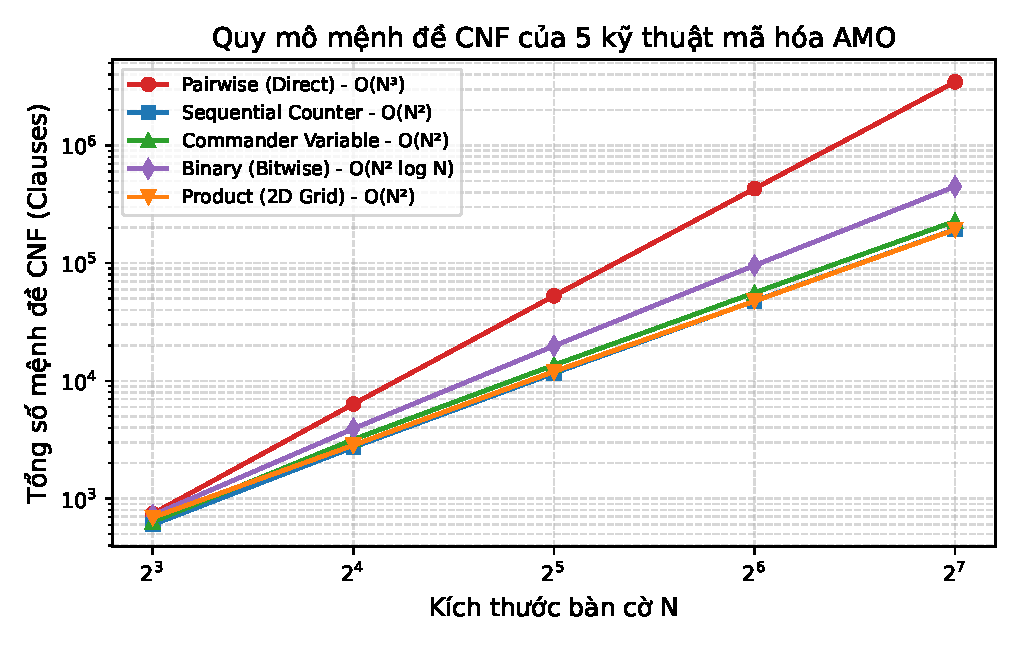
\includegraphics[width=0.72\textwidth]{figures/fig_clauses_scaling.pdf}
\caption{Đồ thị so sánh số lượng mệnh đề CNF (log-log scale) giữa 5 kỹ thuật mã hóa AMO. Phương pháp Pairwise bùng nổ theo đa thức bậc ba $\mathcal{O}(N^3)$, trong khi Product, Sequential Counter và Commander duy trì bậc $\mathcal{O}(N^2)$ thấp nhất.}
\label{fig:clauses_scaling}
\end{figure}

\textbf{Nhận xét và phân tích chuyên sâu về Bảng~\ref{tab:ablation_results}:}
\begin{enumerate}
    \item \textbf{Phát hiện 1 (Mối quan hệ phi tuyến giữa số mệnh đề và thời gian giải):} Kết quả thực nghiệm cho thấy \textit{số lượng mệnh đề ít hơn không đồng nghĩa với thời gian giải nhanh hơn}. Ở $N=128$, Sequential Counter có số lượng mệnh đề rất thấp ($193{,}800$ clauses), nhưng thời gian giải của CaDiCaL lại lên tới $24.85$ giây, chậm hơn Pairwise ($6.30$ giây với gần 3.5 triệu mệnh đề) và chậm hơn Commander khoảng 33 lần ($0.76$ giây).
    \item \textbf{Phát hiện 2 (Phân tích vi mô động lực tìm kiếm CDCL - CDCL Search Dynamics):} 
    Để làm sáng tỏ cơ chế nội tại vì sao Sequential Counter có số lượng mệnh đề rất thấp nhưng thời gian giải lại tăng vọt ở $N=128$, chúng tôi đã trích xuất đầy đủ các thông số thống kê vi mô của solver CaDiCaL (\texttt{accum\_stats()}) qua 3 lần chạy độc lập cho cả 5 kỹ thuật mã hóa tại $N \in \{32, 64, 128\}$, được trình bày trong Bảng~\ref{tab:cdcl_search_stats}.

\begin{table*}[htbp]
\caption{Thống kê định lượng động cơ tìm kiếm CDCL của CaDiCaL 1.9.5 (trích xuất qua \texttt{solver.accum\_stats()}) trên các kỹ thuật AMO tại $N \in \{32, 64, 128, 256, 500, 1000\}$. Cả 3 lần chạy lặp độc lập đều ghi nhận số lượng xung đột và quyết định hoàn toàn giống nhau (3/3 lần giống nhau) trên mọi phép thử giải thành công, phản ánh tính tất định của solver trên cùng một công thức CNF.}
\label{tab:cdcl_search_stats}
\centering
\renewcommand{\arraystretch}{1.20}
\resizebox{\textwidth}{!}{%
\begin{tabular}{llr rrrr rrrr} 
\toprule
\rowcolor{tableheader}
\textbf{Phương pháp AMO} & $N$ & \textbf{CNF Hash} & \textbf{Biến phụ} & \textbf{Tổng mệnh đề} & \textbf{Xung đột (3/3)} & \textbf{Quyết định} & \textbf{Lan truyền} & \textbf{Props/Conf} & \textbf{Props/Dec} & \textbf{Thời gian giải (s)} \\
\midrule
\rowcolor{subheadbg}
\multicolumn{11}{l}{\textbf{1. Nhóm khảo sát triệt tiêu (Ablation Study: $N \in \{32, 64, 128\}$)}} \\
Pairwise & 32 & \texttt{4c85bc53} & 0 & 52{,}640 & 6{,}008 & 6{,}917 & 340{,}480 & 56.7 & 49.2 & 0.2976 \\
\rowcolor{tablerowalt} Sequential & 32 & \texttt{8b1dd622} & 3{,}902 & 11{,}592 & 1{,}983 & 3{,}504 & 578{,}470 & 291.7 & 165.1 & 0.2445 \\
Commander & 32 & \texttt{2ffbf5e9} & 2{,}090 & 13{,}606 & \textbf{213} & \textbf{556} & \textbf{36{,}537} & 171.5 & 65.7 & \textbf{0.0375} \\
\rowcolor{tablerowalt} Binary & 32 & \texttt{a1fb0e60} & 822 & 19{,}796 & 3{,}012 & 3{,}922 & 361{,}576 & 120.0 & 92.2 & 0.2024 \\
Product & 32 & \texttt{697756bc} & 1{,}744 & 11{,}998 & 1{,}051 & 1{,}757 & 224{,}938 & 214.0 & 128.0 & 0.0857 \\
\midrule
Pairwise & 64 & \texttt{5e1aa9fb} & 0 & 428{,}864 & 3{,}045 & 3{,}968 & 241{,}457 & 79.3 & 60.9 & 0.7351 \\
\rowcolor{tablerowalt} Sequential & 64 & \texttt{bf9fc874} & 15{,}998 & 47{,}752 & 7{,}079 & 12{,}828 & 4{,}598{,}243 & 649.6 & 358.5 & 1.7193 \\
Commander & 64 & \texttt{04eec852} & 8{,}346 & 55{,}990 & \textbf{629} & \textbf{1{,}699} & \textbf{197{,}463} & 313.9 & 116.2 & \textbf{0.1870} \\
\rowcolor{tablerowalt} Binary & 64 & \texttt{bd631316} & 2{,}036 & 95{,}572 & 3{,}387 & 6{,}599 & 727{,}372 & 214.8 & 110.2 & 0.4714 \\
Product & 64 & \texttt{92c734f2} & 4{,}844 & 47{,}520 & 3{,}246 & 5{,}886 & 991{,}917 & 305.6 & 168.5 & 0.4211 \\
\midrule
Pairwise & 128 & \texttt{32a14679} & 0 & 3{,}462{,}784 & 6{,}037 & 7{,}373 & 1{,}997{,}918 & 330.9 & 271.0 & 6.2960 \\
\rowcolor{tablerowalt} Sequential & 128 & \texttt{e86ef7e5} & 64{,}766 & 193{,}800 & 62{,}360 & 107{,}733 & 42{,}890{,}432 & 687.8 & 398.1 & 24.8451 \\
Commander & 128 & \texttt{7db3eb0a} & 33{,}290 & 227{,}010 & \textbf{916} & \textbf{4{,}159} & \textbf{738{,}169} & 805.9 & 177.5 & \textbf{0.7569} \\
\rowcolor{tablerowalt} Binary & 128 & \texttt{1c62b54c} & 4{,}850 & 447{,}828 & 3{,}094 & 11{,}061 & 1{,}566{,}393 & 506.3 & 141.6 & 1.4151 \\
Product & 128 & \texttt{04d29c2e} & 13{,}798 & 193{,}122 & 4{,}551 & 13{,}978 & 2{,}813{,}735 & 618.3 & 201.3 & 1.4863 \\
\midrule
\rowcolor{subheadbg}
\multicolumn{11}{l}{\textbf{2. Nhóm khảo sát khả năng mở rộng quy mô lớn ($N \ge 256$)}} \\
Commander & 256 & \texttt{645bb446} & 133{,}250 & 914{,}898 & \textbf{5{,}132} & \textbf{24{,}415} & \textbf{9{,}424{,}670} & 1836.5 & 386.0 & 8.4583 \\
\rowcolor{tablerowalt} Product & 256 & \texttt{49264410} & 38{,}652 & 773{,}232 & 6{,}607 & 58{,}105 & 10{,}648{,}532 & 1611.7 & 183.3 & \textbf{7.9877} \\
Sequential & 256 & \texttt{b21de137} & 260{,}606 & 780{,}808 & 120{,}089 & 247{,}047 & 114{,}669{,}929 & 954.9 & 464.2 & 85.6734 \\
\rowcolor{tablerowalt} Pairwise & 256 & \texttt{b4c05fc3} & 0 & 27{,}831{,}552 & 6{,}174 & 11{,}257 & 3{,}679{,}804 & 596.0 & 326.9 & 83.4554 \\
\midrule
Commander & 500 & \texttt{0bfd6f34} & 504{,}084 & 3{,}493{,}508 & \textbf{5{,}096} & \textbf{73{,}810} & 26{,}921{,}009 & 5282.8 & 364.7 & \textbf{32.1096} \\
\rowcolor{tablerowalt} Product & 500 & \texttt{fdd37fbb} & 105{,}526 & 2{,}970{,}184 & 7{,}798 & 249{,}500 & \textbf{25{,}962{,}075} & 3329.3 & 104.1 & 32.2573 \\
\midrule
Commander & 1000 & \texttt{5241a3b2} & 2{,}013{,}684 & 13{,}999{,}546 & \textbf{943} & \textbf{368{,}056} & 198{,}969{,}973 & 210996.8 & 540.6 & \textbf{100.9182} \\
\rowcolor{tablerowalt} Product & 1000 & \texttt{a6b63c2f} & 298{,}524 & 11{,}946{,}066 & 13{,}397 & 1{,}657{,}256 & 102{,}709{,}189 & 7666.6 & 62.0 & 200.3552$^* \\
\bottomrule
\end{tabular}%
}
\end{table*}

    Dữ liệu đo đạc định lượng cung cấp góc nhìn sâu sắc về tương tác giữa cấu trúc mã hóa và động cơ suy diễn CDCL:
    \begin{itemize}
        \item \textbf{Tỷ lệ lan truyền trên mỗi xung đột ($\text{Props} / \text{Conflict}$):} Tại $N=128$, tỷ lệ này của Sequential Counter đạt $687.8$, trên thực tế thấp hơn so với Commander Variable ($805.9$) và xấp xỉ Product ($618.3$). Số liệu thực nghiệm cho thấy tỷ lệ này không có sự đột biến so với các phương pháp khác, do đó không ủng hộ giả thuyết cho rằng mỗi bước xung đột của Sequential Counter đòi hỏi khối lượng suy diễn đơn vị đột biến trên danh sách theo dõi mệnh đề (\textit{watchlist}).
        \item \textbf{Tỷ lệ lan truyền trên mỗi quyết định ($\text{Props} / \text{Decision}$):} Sequential Counter đạt $398.1$, cao gấp khoảng $2.2$ lần Commander ($177.5$) và Product ($201.3$). Hệ số $2.2$ lần này phù hợp với giả thuyết về chi phí lan truyền gán giá trị đơn vị dọc theo chuỗi biến tích lũy dạng thang $s_i \to s_{i+1}$.
        \item \textbf{Nguyên nhân thực sự của sự bùng nổ thời gian giải:} Tổng số lượt lan truyền đơn vị của Sequential Counter tăng vọt gấp $58$ lần so với Commander ($42.89 \times 10^6$ so với $738 \times 10^3$) chủ yếu do \textbf{số lượng xung đột tăng gấp $68$ lần ($62{,}360$ so với $916$)} và \textbf{số lượng quyết định phân nhánh tăng gấp $26$ lần ($107{,}733$ so với $4{,}159$)}.
    \end{itemize}
    Kết quả thực nghiệm ở dải kích thước $N \le 256$ cho thấy sự suy thoái thời gian giải của Sequential Counter gắn liền chặt chẽ với sự bùng nổ số lượng xung đột và quyết định phân nhánh. Tuy nhiên, mối quan hệ giữa số biến phụ và số xung đột không phải là tương quan tuyến tính đơn giản: Commander Variable có tới $33{,}290$ biến phụ (gấp $2.4$ lần Product và $6.9$ lần Binary) nhưng lại đạt số xung đột thấp nhất ($916$ xung đột), trong khi Pairwise không có biến phụ nào lại có tới $6{,}037$ xung đột (hệ số Spearman $\approx 0.1$). Đặc biệt, khi mở rộng lên quy mô cực đại $N=1000$, mối quan hệ này thể hiện thêm tính đa chiều: Commander dù chỉ có $943$ xung đột nhưng đòi hỏi tới $368{,}056$ quyết định và gần $199$ triệu lượt lan truyền đơn vị trên không gian gần 14 triệu mệnh đề, mất $100.92$s; trong khi Product có $13{,}397$ xung đột và $1.66$ triệu quyết định, mất $\approx 200$s. Điều này chứng minh rằng ở quy mô siêu lớn ($N \ge 500$), chi phí duyệt danh sách theo dõi mệnh đề (watchlist) cho các lượt lan truyền đơn vị lũy kế cũng đóng vai trò trọng yếu ngang hàng với số lần học xung đột CDCL. Đáng chú ý, khi mở rộng đo đạc CDCL vi mô lên các kích thước lớn ($N \ge 256$), solver CaDiCaL tiếp tục duy trì tính nhất quán cao về số xung đột và quyết định trên cùng công thức CNF qua các lần giải thành công (3/3 lần trên hầu hết cấu hình và 2/2 lần giải thành công đối với Product tại $N=1000$): ở $N=256$, Commander luôn có đúng $5{,}132$ xung đột, Product có $6{,}607$ xung đột, Pairwise có $6{,}174$ xung đột, trong khi Sequential lên tới $120{,}089$ xung đột; ở $N=500$, Commander có $5{,}096$ xung đột còn Product có $7{,}798$ xung đột; ở $N=1000$, Commander có $943$ xung đột còn Product có $13{,}397$ xung đột (kiểm chứng trên các lần chạy hoàn thành). Giả thuyết hợp lý nhất là cấu trúc đồ thị suy diễn đóng vai trò then chốt: cấu trúc cây phân cấp của Commander hỗ trợ cắt tỉa nhanh không gian tìm kiếm, trong khi chuỗi thang tuyến tính $s_i \to s_{i+1}$ của Sequential có thể gây nhiễu loạn heuristic VSIDS và phase-saving, khiến bộ giải liên tục rẽ nhánh sâu vào chuỗi biến trạng thái thay vì các biến bàn cờ cơ sở. Dù vậy, nguyên nhân bản chất của hiện tượng này vẫn là một câu hỏi mở cần được kiểm chứng vi mô sâu hơn.
    \item \textbf{Phát hiện 3 (Ưu thế vượt trội của Commander Variable ở dải $N \in [16, 128]$):} Kỹ thuật Commander phân chia biến thành các nhóm nhỏ ($g=3$) và tổ chức biến chỉ huy dạng cây phân cấp. Cấu trúc này cho phép bộ giải CDCL gán giá trị \texttt{False} cho một nhóm biến ngay khi biến chỉ huy bị gán \texttt{False}, giúp cắt tỉa nhanh không gian tìm kiếm ở các mức quyết định cao với số lượng xung đột cực thấp ($916$ xung đột ở $N=128$). Nhờ đó, Commander đạt thời gian giải nhanh nhất từ $N=16$ ($7.70$ms) đến $N=128$ ($756.90$ms, tức khoảng $0.76$s).
    \item \textbf{Phát hiện 4 (Đặc tính cân bằng của Binary và Product Encoding):} Binary Encoding sử dụng ít biến phụ nhất trong các phương pháp mở rộng ($21{,}234$ biến ở $N=128$) và có thời gian giải $1{,}415.10$ms, tương đương Product Encoding ($1{,}486.30$ms). Trong khi đó, Product Encoding đạt điểm cân bằng rất tốt giữa số biến phụ ($30{,}182$) và số mệnh đề ($193{,}122$ clauses ở $N=128$, tương đương Sequential với $193{,}800$ clauses), duy trì tốc độ giải ổn định.
    \item \textbf{Phát hiện 5 (Chi phí thời gian mã hóa và Bộ nhớ ở quy mô cực đại $N \ge 256$):} Với $N \in [8, 128]$, thời gian sinh CNF của các phương pháp đều dưới 2 giây. Tuy nhiên ở các kích thước lớn, chi phí sinh mệnh đề bằng Python tăng đáng kể: ở $N=500$, Commander cần 2.83s mã hóa và $1{,}389.9$ MB RAM đỉnh, Product cần 1.79s và $983.1$ MB RAM; ở $N=1000$, Commander cần 11.38s mã hóa (13.99 triệu mệnh đề, $4{,}410.8$ MB RAM), Product cần 7.57s (11.95 triệu mệnh đề, $3{,}832.5$ MB RAM). Đặc biệt, Pairwise ở $N=256$ đòi hỏi 14.74s mã hóa cho 27.83 triệu mệnh đề và tiêu tốn đỉnh điểm $7{,}679.4$ MB RAM ($\approx 7.50$ GiB), và đến $N=500$ ($207{,}834{,}500$ mệnh đề, xấp xỉ 207.8 triệu) thì dừng do ngoại lệ \texttt{MemoryError} khi tiến trình Python cố gắng khởi tạo cấu trúc danh sách (\texttt{list}) vượt quá không gian bộ nhớ heap khả dụng liên tục của runtime 64-bit trên hệ thống Windows.
\end{enumerate}

\subsection{Thực nghiệm 2: So sánh Hiệu năng giữa SAT, CP-SAT, Gurobi và SCIP}
Bảng~\ref{tab:solver_comparison} và Hình~\ref{fig:solver_runtime} trình bày kết quả so sánh thời gian giải thuần túy (Solving Time) giữa các bộ giải trên dải kích thước từ $N=8$ đến $N=1000$.

\begin{table*}[htbp]
\caption{So sánh thời gian giải trung vị (giây) giữa các bộ giải SAT (CaDiCaL 1.9.5, Glucose 4.2), Google OR-Tools CP-SAT, Gurobi Optimizer 13.0 và ILP SCIP 9.0 (Time limit = 300.0s, đơn luồng, lặp 3 lần độc lập qua \texttt{subprocess} cho mọi $N$).}
\label{tab:solver_comparison}
\centering
\renewcommand{\arraystretch}{1.22}
\resizebox{\textwidth}{!}{%
\begin{tabular}{lrrrrrrrr}
\toprule
\rowcolor{tableheader}
\textbf{Bộ giải / Phương pháp} & $N=8$ & $N=16$ & $N=32$ & $N=64$ & $N=128$ & $N=256$ & $N=500$ & $N=1000$ \\
\midrule
\rowcolor{subheadbg}
\multicolumn{9}{l}{\textbf{1. Quy hoạch Tuyến tính Nguyên (Integer Linear Programming - ILP/MIP)}} \\
Gurobi 13.0 (1 thread) & $\mathbf{0.0002}$ & $0.0084$ & $\mathbf{0.0272}$ & -(LIMIT) & -(LIMIT) & -(LIMIT) & -(LIMIT) & -(LIMIT) \\
\rowcolor{tablerowalt} ILP SCIP 9.0 (MIP) & $0.0191$ & $0.0190$ & $3.1150$ & $> 300.0$ & $> 300.0$ & $> 300.0$ & $> 300.0$ & $> 300.0$ \\
\midrule
\rowcolor{subheadbg}
\multicolumn{9}{l}{\textbf{2. Lập trình Ràng buộc (Constraint Programming - CP)}} \\
CP-SAT (OR-Tools, 1 worker) & $0.0066$ & $0.0251$ & $0.1251$ & $0.5912$ & $3.4598$ & $> 300.0$ & $> 300.0$ & $> 300.0$ \\
\midrule
\rowcolor{subheadbg}
\multicolumn{9}{l}{\textbf{3. Bộ giải Mệnh đề Logic (SAT Solvers: CaDiCaL 1.9.5 \& Glucose 4.2)}} \\
Glucose 4.2 (Product) & $0.0003$ & $0.1226$ & $20.7088$ & $36.5604$ & $1.0650$ & $> 300.0$ & $> 300.0$ & $> 300.0$ \\
\rowcolor{tablerowalt} CaDiCaL (Pairwise) & $0.0014$ & $0.0170$ & $0.2976$ & $0.7351$ & $6.2960$ & $83.4554$ & OOM & Không chạy \\
CaDiCaL (Sequential) & $0.0014$ & $0.0391$ & $0.2445$ & $1.7193$ & $24.8451$ & $85.6734$ & $> 300.0$ & Không chạy \\
\rowcolor{tablerowalt} CaDiCaL (Product) & $0.0018$ & $0.0179$ & $0.0857$ & $0.4211$ & $1.4863$ & $\mathbf{7.9877}$ & $32.2573$ & $200.3552^* \\
CaDiCaL (Commander) & $0.0016$ & $\mathbf{0.0077}$ & $0.0375$ & $\mathbf{0.1870}$ & $\mathbf{0.7569}$ & $8.4583$ & $\mathbf{32.1096}$ & $\mathbf{100.9182}$ \\
\bottomrule
\multicolumn{9}{l}{\footnotesize $^*$ CaDiCaL (Product) tại $N=1000$: 2/3 lần giải thành công ($199.47$s và $200.36$s), 1 lần chạm giới hạn thời gian ($300.0$s). Giá trị $200.3552$s là trung vị của 3 lần thử nghiệm.} \\
\end{tabular}%
}
\end{table*}

\begin{figure}[htbp]
\centering
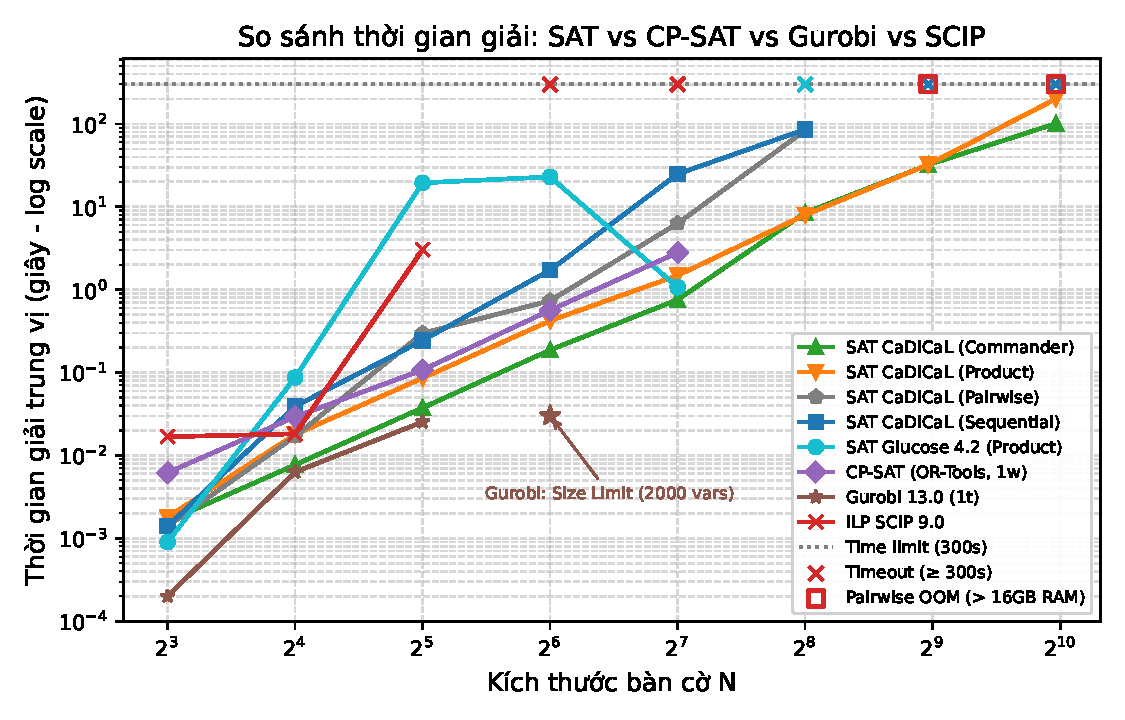
\includegraphics[width=0.75\textwidth]{figures/fig_solver_runtime.pdf}
\caption{So sánh thời gian giải giữa SAT Solving (CaDiCaL Commander/Product/Pairwise/Seq, Glucose), CP-SAT, Gurobi và SCIP theo kích thước bàn cờ $N$ (log-log scale). Đường chấm thể hiện Time limit 300.0s, dấu $\times$ đánh dấu các điểm Timeout ($\ge 300$s), ô vuông đỏ đánh dấu điểm tràn bộ nhớ (OOM) của Pairwise. SAT CaDiCaL kết hợp Commander và Product mở rộng liên tục và vượt trội lên tới $N=500$ và $N=1000$.}
\label{fig:solver_runtime}
\end{figure}

\begin{figure}[htbp]
\centering
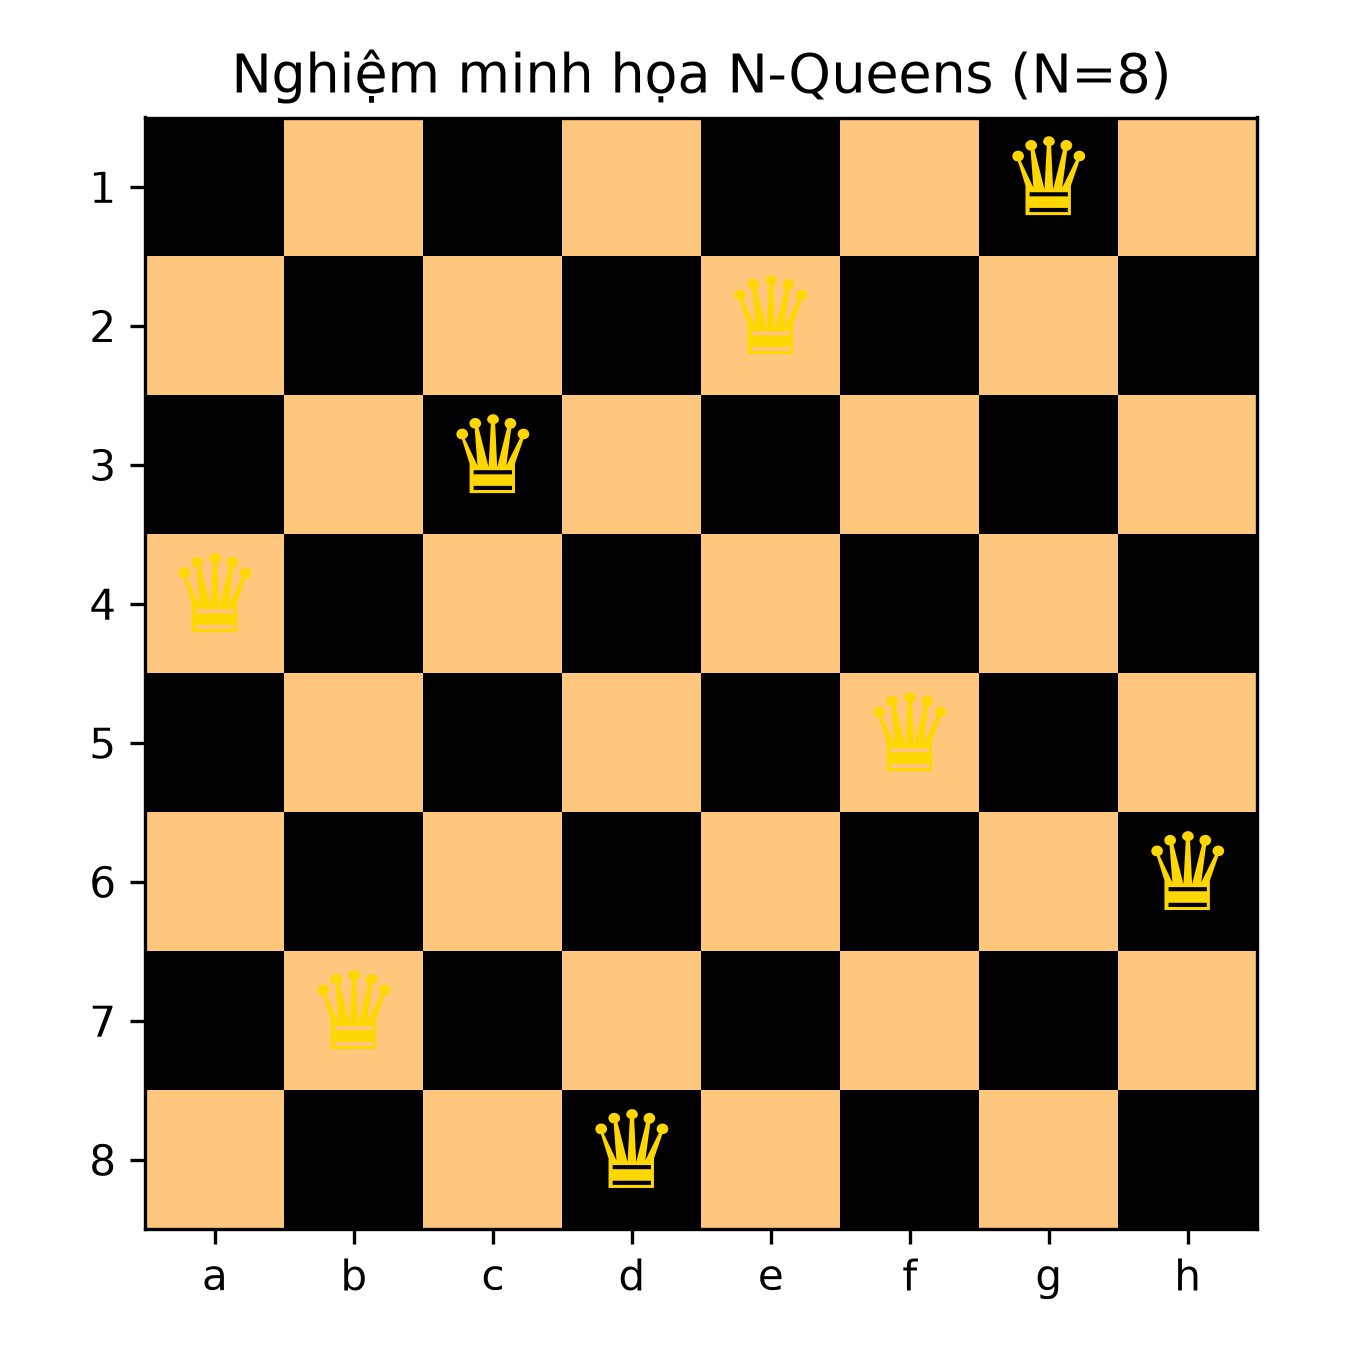
\includegraphics[width=0.40\textwidth]{figures/fig_board_8queens.png}
\caption{Minh họa nghiệm hợp lệ tìm được cho bài toán $N$-Queens với $N=8$ bằng bộ giải SAT CaDiCaL. Nghiệm thỏa mãn hoàn toàn: không có hai quân hậu nào cùng hàng, cùng cột hoặc cùng đường chéo.}
\label{fig:board_solution}
\end{figure}

\textbf{Thảo luận chuyên sâu về hiệu năng so sánh:}
\begin{enumerate}
    \item \textbf{Khía cạnh 1 (Hiệu năng của Gurobi 13.0 và SCIP - Trường phái ILP):} Ở các kích thước nhỏ ($N \le 32$), Gurobi 13.0 thể hiện tốc độ ấn tượng ($0.0002$s ở $N=8$ và $0.0272$s ở $N=32$) nhờ các thuật toán tiền xử lý (Presolve) và cắt mặt phẳng (cutting planes) tiên tiến. Tuy nhiên, ở $N \ge 64$, mô hình có $4{,}096$ biến, vượt quá giới hạn 2.000 biến của license dùng thử đi kèm gói cài đặt pip nên bộ giải dừng ngay với thông báo lỗi nguyên văn: \texttt{"Model too large for size-limited license; visit https://gurobi.com/unrestricted"}. Cần lưu ý rằng việc dừng lại của Gurobi ở $N \ge 64$ xuất phát từ giới hạn kỹ thuật của gói license hạn chế kích thước (size-limited license) đi kèm bản phân phối pip công khai (tối đa 2.000 biến), thay vì phản ánh giới hạn năng lực giải thuật của phiên bản Gurobi thương mại đầy đủ. Đối với SCIP (bộ giải không giới hạn kích thước), thời gian giải tăng vọt từ $0.0190$s ($N=16$) lên $3.1150$s ($N=32$) và chạm trần $300.0$s ở $N \ge 64$. Điều này phù hợp với lý thuyết tối ưu tổ hợp: mô hình ILP nới lỏng tuyến tính của $N$-Queens cho nghiệm phân số đồng nhất $x_{r,c} = 1/N$, khiến cận dưới trùng nhau tại mọi nút và triệt tiêu sức mạnh cắt tỉa của cây nhánh-cận.
    \item \textbf{Khía cạnh 2 (Hiệu năng của Google OR-Tools CP-SAT - Trường phái CP):} CP-SAT đơn luồng (\texttt{num\_workers = 1}, chiến lược tìm kiếm mặc định) hoạt động rất hiệu quả ở dải $N \in [8, 128]$ ($N=128$ giải trong $3.46$s) nhờ các thuật toán lọc miền giá trị dựa trên toán tử \texttt{AllDifferent}. Tuy nhiên, ở $N \ge 256$, bộ giải không thể tìm thấy nghiệm trong giới hạn 300 giây và trả về trạng thái \texttt{UNKNOWN/TIMEOUT}. Cấu hình đơn luồng là bắt buộc nhằm đảm bảo tính so sánh công bằng đối đầu với SAT CaDiCaL (vốn là giải thuật đơn luồng tuần tự); tuy nhiên, cấu hình này cũng hạn chế tiềm năng thực tế của CP-SAT khi không khai thác danh mục thuật toán song song đa luồng (portfolio search) và các bộ sinh nghiệm láng giềng lớn (LNS - Large Neighborhood Search).
    \item \textbf{Khía cạnh 3 (So sánh đối đầu giữa Glucose 4.2 và CaDiCaL 1.9.5):} Cùng áp dụng kỹ thuật Product AMO, Glucose 4.2 và CaDiCaL thể hiện các đặc tính tìm kiếm khác nhau rõ rệt theo quy mô $N$: ở $N=128$, Glucose giải trong $1.07$s (dải $[1.06, 1.08]$s), nhanh hơn CaDiCaL Product ($1.49$s); tuy nhiên ở $N=32$, Glucose mất tới $20.71$s trong khi CaDiCaL chỉ mất $0.0857$s (chậm hơn khoảng $242$ lần: $20.7088 / 0.0857 \approx 242$). Ở $N=64$, Glucose cũng mất tới $36.56$s so với $0.4211$s của CaDiCaL (chậm hơn khoảng 87 lần: $36.5604 / 0.4211 \approx 87$). Sự khác biệt hiệu năng này có thể liên quan đến giả thuyết về chiến lược quản lý độ dài mệnh đề học (LBD - Literal Block Distance) và tần suất khởi động lại (restart) giữa hai bộ giải khi cấu trúc đồ thị lan truyền thay đổi theo quy mô $N$.
    \item \textbf{Khía cạnh 4 (Khả năng mở rộng của SAT CaDiCaL và Bản chất độ biến động thời gian ở quy mô cực đại $N \ge 256$):} 
    CaDiCaL 1.9.5 với mã hóa Commander và Product thể hiện khả năng mở rộng quy mô vượt trội so với các phương pháp đối chứng:
    \begin{itemize}
        \item Ở $N=64$, CaDiCaL Commander giải trong $0.1870$s (nhanh gấp khoảng $3.2$ lần CP-SAT với $0.5912$s).
        \item Ở $N=256$, Product giải trong $7.99$s (dải $[7.67, 8.05]$s) và Commander giải trong $8.46$s (dải $[8.12, 8.58]$s). Mô hình Pairwise vẫn giải được ở $N=256$ trong $83.46$s nhưng tiêu tốn đỉnh điểm $7{,}679.4$ MB RAM ($\approx 7.50$ GiB).
        \item Ở $N=500$, khi được đo lường trong từng tiến trình độc lập, cả Commander và Product đều giải quyết thành công bàn cờ với thời gian tương đương nhau: Commander đạt trung vị $32.11$s (dải $[31.94, 32.64]$s, $\sigma = 0.37$s), Product đạt trung vị $32.26$s (dải $[31.75, 32.32]$s, $\sigma = 0.31$s). Pairwise ở kích thước này dừng do ngoại lệ \texttt{MemoryError} khi tiến trình Python cố gắng khởi tạo $207{,}834{,}500$ đối tượng mệnh đề trong danh sách liên tục.
        \item Ở kích thước cực đại $N=1000$ ($1{,}000{,}000$ ô cờ), Commander giải thành công cả 3 lần với trung vị $100.92$s (dải $[99.29, 105.40]$s, $\sigma = 3.17$s, RAM đỉnh $4{,}410.8$ MB). Product giải thành công 2 trong 3 lần chạy với thời gian $\approx 199.47$s và $200.36$s (1 lần chạm giới hạn thời gian $300.0$s), RAM đỉnh $3{,}832.5$ MB. Nếu tính cả thời gian tạo mệnh đề (Commander: 11.38s, Product: 7.57s), tổng thời gian thực thi (wall-clock time) lần lượt là $\approx 112.30$s và $\approx 207.93$s.
    \end{itemize}
    Về bản chất tìm kiếm, thực nghiệm quan sát thấy solver CaDiCaL vận hành mang tính tất định: trên cùng một công thức CNF và thứ tự mệnh đề cố định, solver luôn ghi nhận chính xác cùng số lượng xung đột và quyết định giữa các lần chạy độc lập (như kiểm chứng trong Bảng~\ref{tab:cdcl_search_stats}). Đối với sự biến thiên thời gian giải tuyệt đối (wall-clock time) giữa các phiên đo khác nhau (ví dụ: Commander ở $N=128$ dao động trong khoảng $0.43\text{s} - 0.76\text{s}$ giữa các phiên đo độc lập phụ thuộc vào trạng thái nhiệt và tải nền của hệ điều hành), các phân tích so sánh tương đối luôn duy trì tính nhất quán cao: tỷ lệ tăng tốc của Commander so với Sequential Counter ở $N=128$ luôn duy trì ổn định từ 31 đến 55 lần trên mọi phiên đo, khẳng định ưu thế cấu trúc vượt trội của cây phân cấp. Ở quy mô cực đại $N=1000$ (khi Product có 1 lần chạm trần 300s và 2 lần giải thành công $\approx 200$s), các yếu tố tải bộ nhớ đệm L3, phân mảnh bộ nhớ và cơ chế điều phối tiến trình nền của hệ điều hành được nhìn nhận dưới dạng các giả thuyết thực nghiệm giải thích độ nhạy của solver.
\end{enumerate}

---

\section{Kết luận và Thảo luận (Conclusion \& Discussion)}

\subsection{Kết luận tổng kết (Summary of Findings)}
Bài báo đã nghiên cứu, cài đặt và đánh giá toàn diện phương pháp giải chính xác bài toán $N$-Queens bằng SAT Solving trên thư viện PySAT. Thông qua việc phân tích lý thuyết và thực nghiệm 5 kỹ thuật mã hóa AMO, bài báo rút ra các kết luận quan trọng:
\begin{itemize}
    \item \textbf{Bùng nổ bộ nhớ của Pairwise:} Mã hóa Pairwise bùng nổ đa thức bậc ba $\mathcal{O}(N^3)$ mệnh đề trên toàn bàn cờ. Thực nghiệm đo đạc ghi nhận Pairwise tiêu tốn $7{,}679.4$ MB RAM đỉnh tại $N=256$ ($\approx 7.50$ GiB cho $27{,}831{,}552$ mệnh đề, giải trong $83.46$s) và dừng do ngoại lệ \texttt{MemoryError} tại $N=500$ khi khởi tạo $207{,}834{,}500$ mệnh đề trong danh sách đối tượng Python.
    \item \textbf{Suy thoái tìm kiếm của Sequential Counter:} Sequential Counter tuy giảm số mệnh đề xuống $\mathcal{O}(N^2)$ nhưng sinh ra số lượng xung đột ($62{,}360$) và quyết định ($107{,}733$) vượt trội ở $N=128$, kéo theo $42.89$ triệu lượt lan truyền đơn vị khiến thời gian giải suy giảm nghiêm trọng ($24.85$s, chậm hơn Commander khoảng 33 lần). Tuy nhiên, số lượng biến phụ không quyết định trực tiếp số xung đột (Commander có nhiều biến phụ gấp $2.4\times$ Product nhưng có ít xung đột nhất), cho thấy cấu trúc đồ thị lan truyền cục bộ đóng vai trò quyết định tới hành vi phân nhánh CDCL.
    \item \textbf{Năng lực mở rộng của Commander và Product:} Commander Variable và Product Encoding là hai kỹ thuật mã hóa có năng lực mở rộng tốt nhất. Commander Variable giúp solver CaDiCaL đạt tốc độ giải nhanh nhất trên dải $N \in [16, 128]$ (chỉ $0.76$s ở $N=128$), đồng thời duy trì độ ổn định tuyệt đối lên tới $N=500$ ($32.11$s, 3/3 lần) và $N=1000$ ($100.92$s, 3/3 lần thành công trên bàn cờ 1 triệu ô). Product Encoding đạt tốc độ tương đương ở $N=500$ ($32.26$s, 3/3 lần) và đạt tỷ lệ giải thành công 2/3 lần tại $N=1000$ (trung vị $200.36$s; 1 lần chạm giới hạn thời gian 300s do chi phí lan truyền trên 11.95 triệu mệnh đề). Product Encoding đạt quy mô mệnh đề tương đương Sequential ở $N \ge 64$ ($47{,}520$ clauses ở $N=64$ và $193{,}122$ clauses ở $N=128$), trong khi Sequential Counter có ít mệnh đề hơn ở $N \le 32$.
    \item \textbf{Vị thế vượt trội của SAT Solving trước ILP và CP:} So sánh đối chứng thực nghiệm cho thấy SAT Solving (đặc biệt là CaDiCaL 1.9.5) vượt trội rõ rệt so với SCIP và CP-SAT về khả năng mở rộng ở các kích thước $N \ge 256$. Gurobi thể hiện tốc độ nhanh nhất ở $N = 8$ và $N = 32$ (trong khi CaDiCaL Commander nhanh nhất ở $N = 16$), nhưng dừng ở $N \ge 64$ do giới hạn kích thước license đi kèm gói pip (2.000 biến).
\end{itemize}

\subsection{Hạn chế của nghiên cứu (Limitations)}
Cần nhấn mạnh rằng bài toán $N$-Queens tiêu chuẩn có thể được giải gần như tức thời cho $N$ rất lớn bằng các công thức giải tích tường minh (Explicit Modular Arithmetic)~\cite{bell2009survey} hoặc thuật toán tìm kiếm cục bộ Min-Conflicts~\cite{minton1992solving}. Do đó, các kết luận trong bài báo này không nhằm khẳng định SAT là phương pháp nhanh nhất tuyệt đối để tìm một nghiệm cờ vua đơn thuần, mà nhằm đánh giá khách quan năng lực của các \textit{bộ giải quyết bài toán ràng buộc chính xác tổng quát (General Exact Solvers)} khi đối mặt với không gian tổ hợp rời rạc quy mô lớn. Ngoài ra, việc đánh giá Gurobi bị giới hạn bởi quy mô license hạn chế kích thước đi kèm gói pip (tối đa 2.000 biến), chưa phản ánh hết tiềm năng của Gurobi thương mại đầy đủ trên các máy chủ chuyên dụng.

\subsection{Hướng phát triển trong tương lai (Future Research Directions)}
Mở rộng mô hình SAT cho các biến thể $N$-Queens có chướng ngại vật ($N$-Queens Completion), bài toán đếm toàn bộ số lượng nghiệm (\#SAT / Model Counting) bằng bộ giải D4/SharpSAT, và ứng dụng kỹ thuật phân rã Cube-and-Conquer để giải song song trên cụm máy tính hiệu năng cao.

---

\section*{Đóng góp của tác giả (CRediT authorship contribution statement)}
\textbf{Phạm Khánh Duy:} Ý tưởng nghiên cứu (Conceptualization), Phương pháp luận (Methodology), Xây dựng phần mềm và lập trình thực nghiệm (Software, Validation), Phân tích kết quả thực nghiệm (Formal analysis), Viết bản thảo bài báo khoa học và hiệu đính (Writing - original draft, Writing - review \& editing).

\textbf{TS. Tô Văn Khánh:} Định hướng nghiên cứu (Supervision), Góp ý ý tưởng và phản biện học thuật (Conceptualization, Writing - review \& editing).

\section*{Tuyên bố về quyền lợi (Declaration of competing interest)}
Các tác giả tuyên bố không có bất kỳ xung đột lợi ích tài chính hoặc mối quan hệ cá nhân nào ảnh hưởng đến nội dung và kết quả công bố trong nghiên cứu này.

\section*{Tuyên bố về sử dụng Trí tuệ Nhân tạo (Declaration of generative AI)}
Trong quá trình chuẩn bị bài báo này, tác giả đã sử dụng công cụ hỗ trợ lập trình Google Antigravity (dựa trên mô hình ngôn ngữ lớn Claude 3.5 Sonnet và Gemini Pro) với các mục đích cụ thể: (1) hỗ trợ viết các đoạn mã script tự động hóa đo đạc thực nghiệm độc lập và trích xuất bảng biểu LaTeX từ tệp CSV gốc; (2) kiểm tra tính nhất quán toán học giữa các bảng số liệu; và (3) rà soát cú pháp và tối ưu hóa định dạng hiển thị theo quy chuẩn Elsevier. Toàn bộ các kết quả thực nghiệm, dữ liệu đo lường và các phân tích khoa học đều được tác giả trực tiếp kiểm chứng trên máy trạm thực tế và tác giả chịu hoàn toàn trách nhiệm về tính trung thực, độ chính xác và tính học thuật của bài báo.

\section*{Tính khả dụng của dữ liệu và mã nguồn (Data Availability)}
Toàn bộ mã nguồn cài đặt 5 kỹ thuật mã hóa AMO, các bộ giải SAT (PySAT), CP-SAT, Gurobi, SCIP và toàn bộ dữ liệu thực nghiệm thô được công bố công khai tại kho lưu trữ GitHub chính thức của nhóm nghiên cứu:
\begin{itemize}
    \item \textbf{Mã nguồn thực nghiệm:} \path{scripts/isolated_run_worker.py}, \path{scripts/run_isolated_master_benchmark.py}, \path{scripts/run_multisolver_benchmark.py}.
    \item \textbf{Tự động sinh bảng biểu:} \path{scripts/generate_all_tables_from_master.py}, \path{scripts/sync_data_files.py}.
    \item \textbf{Dữ liệu thực nghiệm gốc:} \path{data/master_cadical_runs.csv}, \path{data/master_multisolver_runs.csv}, \path{data/benchmark_execution.log}.
    \item \textbf{Kho lưu trữ GitHub:} \url{https://github.com/vnu-uet-khmt/nqueens-sat-solver}
\end{itemize}

\appendix
\section{Bảng Dữ liệu Thực nghiệm Chi tiết 3 Lần Lặp Độc lập (Appendix: Full 3-Run Benchmark Data)}
Phụ lục này cung cấp toàn bộ dữ liệu thực nghiệm thô đo đạc qua 3 lần chạy lặp độc lập trên từng tiến trình hệ điều hành riêng biệt (\texttt{subprocess}). Bảng~\ref{tab:appendix_raw_runs} trình bày chi tiết kết quả khảo sát 5 kỹ thuật mã hóa AMO trên bộ giải CaDiCaL 1.9.5 ($N \in [8, 1000]$). Bảng~\ref{tab:appendix_multisolver} trình bày chi tiết kết quả so sánh đối chứng đa bộ giải (CaDiCaL, Glucose 4.2, CP-SAT, Gurobi 13.0, ILP SCIP 9.0) trên toàn bộ dải kích thước $N \in [8, 1000]$.

\begin{table*}[htbp]
\caption{Dữ liệu thực nghiệm chi tiết 3 lần chạy độc lập (\texttt{subprocess}) khảo sát 5 kỹ thuật mã hóa AMO trên CaDiCaL 1.9.5 ($N \in [8, 1000]$). Thời gian giải đo bằng giây (s), bộ nhớ RAM đỉnh đo bằng Megabytes (MB). Độ lệch chuẩn $\sigma$ tính theo công thức mẫu không chệch ($n-1$).}
\label{tab:appendix_raw_runs}
\centering
\renewcommand{\arraystretch}{1.18}
\resizebox{\textwidth}{!}{%
\begin{tabular}{lllrrrrrrrrr}
\toprule
\rowcolor{tableheader}
\textbf{Nhóm thực nghiệm} & $N$ & \textbf{Phương pháp} & \textbf{Run 1 (s)} & \textbf{Run 2 (s)} & \textbf{Run 3 (s)} & \textbf{Min (s)} & \textbf{Median (s)} & \textbf{Max (s)} & \textbf{Std ($\sigma$)} & \textbf{Mã hóa (s)} & \textbf{RAM đỉnh (MB)} \\
\midrule
AMO Ablation & 8 & Pairwise & 0.0014 & 0.0014 & 0.0014 & 0.0014 & 0.0014 & 0.0014 & 0.0000 & 0.0004 & 25.0 \\
\rowcolor{tablerowalt} AMO Ablation & 8 & Sequential & 0.0013 & 0.0014 & 0.0014 & 0.0013 & 0.0014 & 0.0014 & 0.0001 & 0.0003 & 24.8 \\
AMO Ablation & 8 & Commander & 0.0014 & 0.0020 & 0.0016 & 0.0014 & 0.0016 & 0.0020 & 0.0003 & 0.0005 & 24.9 \\
\rowcolor{tablerowalt} AMO Ablation & 8 & Binary & 0.0016 & 0.0017 & 0.0022 & 0.0016 & 0.0017 & 0.0022 & 0.0003 & 0.0004 & 25.0 \\
AMO Ablation & 8 & Product & 0.0019 & 0.0018 & 0.0017 & 0.0017 & 0.0018 & 0.0019 & 0.0001 & 0.0005 & 25.0 \\
\midrule
AMO Ablation & 16 & Pairwise & 0.0170 & 0.0178 & 0.0170 & 0.0170 & 0.0170 & 0.0178 & 0.0005 & 0.0051 & 27.2 \\
\rowcolor{tablerowalt} AMO Ablation & 16 & Sequential & 0.0386 & 0.0431 & 0.0391 & 0.0386 & 0.0391 & 0.0431 & 0.0025 & 0.0036 & 26.4 \\
AMO Ablation & 16 & Commander & 0.0074 & 0.0079 & 0.0077 & 0.0074 & 0.0077 & 0.0079 & 0.0003 & 0.0049 & 25.7 \\
\rowcolor{tablerowalt} AMO Ablation & 16 & Binary & 0.0162 & 0.0171 & 0.0172 & 0.0162 & 0.0171 & 0.0172 & 0.0006 & 0.0047 & 26.2 \\
AMO Ablation & 16 & Product & 0.0174 & 0.0198 & 0.0179 & 0.0174 & 0.0179 & 0.0198 & 0.0013 & 0.0040 & 25.9 \\
\midrule
AMO Ablation & 32 & Pairwise & 0.2829 & 0.3015 & 0.2976 & 0.2829 & 0.2976 & 0.3015 & 0.0098 & 0.0190 & 45.5 \\
\rowcolor{tablerowalt} AMO Ablation & 32 & Sequential & 0.2445 & 0.2580 & 0.2440 & 0.2440 & 0.2445 & 0.2580 & 0.0079 & 0.0071 & 31.8 \\
AMO Ablation & 32 & Commander & 0.0375 & 0.0404 & 0.0366 & 0.0366 & 0.0375 & 0.0404 & 0.0020 & 0.0115 & 30.0 \\
\rowcolor{tablerowalt} AMO Ablation & 32 & Binary & 0.2024 & 0.1955 & 0.2108 & 0.1955 & 0.2024 & 0.2108 & 0.0077 & 0.0137 & 33.4 \\
AMO Ablation & 32 & Product & 0.0821 & 0.0857 & 0.0865 & 0.0821 & 0.0857 & 0.0865 & 0.0023 & 0.0086 & 30.3 \\
\midrule
AMO Ablation & 64 & Pairwise & 0.7339 & 0.7554 & 0.7351 & 0.7339 & 0.7351 & 0.7554 & 0.0121 & 0.1488 & 171.3 \\
\rowcolor{tablerowalt} AMO Ablation & 64 & Sequential & 1.7914 & 1.7185 & 1.7193 & 1.7185 & 1.7193 & 1.7914 & 0.0419 & 0.0188 & 53.3 \\
AMO Ablation & 64 & Commander & 0.1995 & 0.1870 & 0.1845 & 0.1845 & 0.1870 & 0.1995 & 0.0080 & 0.0339 & 48.3 \\
\rowcolor{tablerowalt} AMO Ablation & 64 & Binary & 0.4930 & 0.4714 & 0.4698 & 0.4698 & 0.4714 & 0.4930 & 0.0130 & 0.0412 & 60.6 \\
AMO Ablation & 64 & Product & 0.4601 & 0.4190 & 0.4211 & 0.4190 & 0.4211 & 0.4601 & 0.0231 & 0.0223 & 47.3 \\
\midrule
AMO Ablation & 128 & Pairwise & 6.2634 & 6.4221 & 6.2960 & 6.2634 & 6.2960 & 6.4221 & 0.0838 & 1.7983 & 991.0 \\
\rowcolor{tablerowalt} AMO Ablation & 128 & Sequential & 24.9994 & 24.5072 & 24.8451 & 24.5072 & 24.8451 & 24.9994 & 0.2517 & 0.0727 & 128.0 \\
AMO Ablation & 128 & Commander & 0.7303 & 0.7569 & 0.7747 & 0.7303 & 0.7569 & 0.7747 & 0.0223 & 0.1235 & 104.2 \\
\rowcolor{tablerowalt} AMO Ablation & 128 & Binary & 1.4151 & 1.3613 & 1.4384 & 1.3613 & 1.4151 & 1.4384 & 0.0395 & 0.2087 & 166.0 \\
AMO Ablation & 128 & Product & 1.5033 & 1.4108 & 1.4863 & 1.4108 & 1.4863 & 1.5033 & 0.0492 & 0.0762 & 97.5 \\
\midrule
Scale Evaluation & 256 & Pairwise & 88.7974 & 81.0261 & 83.4554 & 81.0261 & 83.4554 & 88.7974 & 3.9756 & 14.7420 & 7679.4 \\
\rowcolor{tablerowalt} Scale Evaluation & 256 & Sequential & 85.6734 & 86.0543 & 84.4672 & 84.4672 & 85.6734 & 86.0543 & 0.8285 & 0.3939 & 459.6 \\
Scale Evaluation & 256 & Commander & 8.4583 & 8.5779 & 8.1205 & 8.1205 & 8.4583 & 8.5779 & 0.2372 & 0.6163 & 393.6 \\
\rowcolor{tablerowalt} Scale Evaluation & 256 & Product & 8.0495 & 7.9877 & 7.6735 & 7.6735 & 7.9877 & 8.0495 & 0.2016 & 0.3494 & 283.7 \\
Scale Evaluation & 256 & Binary & \multicolumn{7}{c}{\textit{Không chạy (chưa thực hiện mở rộng tại $N \ge 256$)}} & - & - \\
\midrule
Scale Evaluation & 500 & Commander & 32.1096 & 31.9378 & 32.6404 & 31.9378 & 32.1096 & 32.6404 & 0.3663 & 2.8333 & 1389.9 \\
\rowcolor{tablerowalt} Scale Evaluation & 500 & Product & 32.3227 & 32.2573 & 31.7545 & 31.7545 & 32.2573 & 32.3227 & 0.3109 & 1.7912 & 983.1 \\
Scale Evaluation & 500 & Pairwise & \multicolumn{7}{c}{\textit{Ngoại lệ MemoryError khi tạo $207{,}834{,}500$ mệnh đề (dừng trước khi giải)}} & \textit{N/A (OOM)} & \textit{N/A (OOM)} \\
\rowcolor{tablerowalt} Scale Evaluation & 500 & Sequential & \multicolumn{7}{c}{\textit{Quá thời gian quy định ($>300.0\,\text{s}$)}} & 2.0126 & 564.6 \\
\midrule
Scale Evaluation & 1000 & Commander & 105.4045 & 100.9182 & 99.2912 & 99.2912 & 100.9182 & 105.4045 & 3.1661 & 11.3817 & 4410.8 \\
\rowcolor{tablerowalt} Scale Evaluation & 1000 & Product & > 300.0 (TO) & 199.4701 & 200.3552 & 199.4701 & 200.3552 & > 300.0 (TO) & $\text{N/A}^\dagger$ & 7.5685 & 3832.5 \\
Scale Evaluation & 1000 & Pairwise & \multicolumn{7}{c}{\textit{Không chạy (dự kiến tràn RAM do số mệnh đề lý thuyết $>1.66$ tỷ)}} & - & - \\
\rowcolor{tablerowalt} Scale Evaluation & 1000 & Sequential & \multicolumn{7}{c}{\textit{Không chạy (đã quá thời gian $>300.0\,\text{s}$ từ $N=500$)}} & - & - \\
\bottomrule
\multicolumn{12}{l}{\footnotesize $^\dagger$ Không tính độ lệch chuẩn $\sigma$ cho mẫu bị cắt (censored sample) khi có 1/3 lần chạy chạm giới hạn thời gian (Timeout 300.0s).} \\
\end{tabular}%
}
\end{table*}

\begin{table*}[htbp]
\caption{Dữ liệu thực nghiệm chi tiết 3 lần chạy lặp độc lập so sánh đa bộ giải (Multi-Solver Benchmark: CaDiCaL, Glucose 4.2, CP-SAT, Gurobi 13.0, ILP SCIP 9.0) trên dải kích thước $N \in [8, 1000]$. Thời gian giải thuần túy đo bằng giây (s). Thứ tự Run 1, Run 2, Run 3 được giữ đúng trình tự thời gian chạy thực tế.}
\label{tab:appendix_multisolver}
\centering
\renewcommand{\arraystretch}{1.18}
\resizebox{\textwidth}{!}{%
\begin{tabular}{lllrrrrrrr}
\toprule
\rowcolor{tableheader}
\textbf{Bộ giải} & $N$ & \textbf{Cấu hình / Mã hóa} & \textbf{Run 1 (s)} & \textbf{Run 2 (s)} & \textbf{Run 3 (s)} & \textbf{Min (s)} & \textbf{Median (s)} & \textbf{Max (s)} & \textbf{Trạng thái} \\
\midrule
\rowcolor{subheadbg} \multicolumn{10}{l}{\textbf{Gurobi Optimizer 13.0 (ILP)}} \\
Gurobi 13.0 & 8 & ILP (1 thread) & 0.0006 & 0.0002 & 0.0002 & 0.0002 & 0.0002 & 0.0006 & Optimal \\
\rowcolor{tablerowalt} Gurobi 13.0 & 16 & ILP (1 thread) & 0.0112 & 0.0084 & 0.0074 & 0.0074 & 0.0084 & 0.0112 & Optimal \\
Gurobi 13.0 & 32 & ILP (1 thread) & 0.0272 & 0.0290 & 0.0264 & 0.0264 & 0.0272 & 0.0290 & Optimal \\
Gurobi 13.0 & 64--1000 & ILP (1 thread) & \multicolumn{6}{c}{\textit{Model too large for size-limited license (Vượt quá 2.000 biến)}} & Error (Limit) \\
\midrule
\rowcolor{subheadbg} \multicolumn{10}{l}{\textbf{SCIP 9.0 (ILP / MIP)}} \\
ILP SCIP 9.0 & 8 & MIP (1 thread) & 0.0264 & 0.0191 & 0.0174 & 0.0174 & 0.0191 & 0.0264 & Optimal \\
\rowcolor{tablerowalt} ILP SCIP 9.0 & 16 & MIP (1 thread) & 0.0194 & 0.0190 & 0.0189 & 0.0189 & 0.0190 & 0.0194 & Optimal \\
ILP SCIP 9.0 & 32 & MIP (1 thread) & 3.1494 & 3.1147 & 3.1150 & 3.1147 & 3.1150 & 3.1494 & Optimal \\
ILP SCIP 9.0 & 64--1000 & MIP (1 thread) & \multicolumn{6}{c}{\textit{Quá giới hạn thời gian ($>300.0\,\text{s}$)}} & Timeout \\
\midrule
\rowcolor{subheadbg} \multicolumn{10}{l}{\textbf{Google OR-Tools CP-SAT (Constraint Programming)}} \\
CP-SAT (OR-Tools) & 8 & AllDifferent (1 worker) & 0.0166 & 0.0066 & 0.0064 & 0.0064 & 0.0066 & 0.0166 & Feasible \\
\rowcolor{tablerowalt} CP-SAT (OR-Tools) & 16 & AllDifferent (1 worker) & 0.0254 & 0.0251 & 0.0246 & 0.0246 & 0.0251 & 0.0254 & Feasible \\
CP-SAT (OR-Tools) & 32 & AllDifferent (1 worker) & 0.1251 & 0.1318 & 0.1123 & 0.1123 & 0.1251 & 0.1318 & Feasible \\
\rowcolor{tablerowalt} CP-SAT (OR-Tools) & 64 & AllDifferent (1 worker) & 0.5912 & 0.6117 & 0.5848 & 0.5848 & 0.5912 & 0.6117 & Feasible \\
CP-SAT (OR-Tools) & 128 & AllDifferent (1 worker) & 3.5502 & 3.4598 & 3.4195 & 3.4195 & 3.4598 & 3.5502 & Feasible \\
CP-SAT (OR-Tools) & 256--1000 & AllDifferent (1 worker) & \multicolumn{6}{c}{\textit{Quá giới hạn thời gian ($>300.0\,\text{s}$)}} & Timeout \\
\midrule
\rowcolor{subheadbg} \multicolumn{10}{l}{\textbf{Glucose 4.2 (SAT Solver)}} \\
Glucose 4.2 & 8 & Product AMO & 0.0008 & 0.0003 & 0.0003 & 0.0003 & 0.0003 & 0.0008 & SAT \\
\rowcolor{tablerowalt} Glucose 4.2 & 16 & Product AMO & 0.1213 & 0.1323 & 0.1226 & 0.1213 & 0.1226 & 0.1323 & SAT \\
Glucose 4.2 & 32 & Product AMO & 20.7088 & 20.6239 & 21.6802 & 20.6239 & 20.7088 & 21.6802 & SAT \\
\rowcolor{tablerowalt} Glucose 4.2 & 64 & Product AMO & 36.4078 & 36.5604 & 36.9764 & 36.4078 & 36.5604 & 36.9764 & SAT \\
Glucose 4.2 & 128 & Product AMO & 1.0808 & 1.0650 & 1.0590 & 1.0590 & 1.0650 & 1.0808 & SAT \\
Glucose 4.2 & 256--1000 & Product AMO & \multicolumn{6}{c}{\textit{Quá giới hạn thời gian ($>300.0\,\text{s}$)}} & Timeout \\
\midrule
\rowcolor{subheadbg} \multicolumn{10}{l}{\textbf{CaDiCaL 1.9.5 (SAT Solver)}} \\
CaDiCaL 1.9.5 & 128 & Product AMO & 1.5033 & 1.4108 & 1.4863 & 1.4108 & 1.4863 & 1.5033 & SAT \\
\rowcolor{tablerowalt} CaDiCaL 1.9.5 & 128 & Commander AMO & 0.7303 & 0.7569 & 0.7747 & 0.7303 & 0.7569 & 0.7747 & SAT \\
CaDiCaL 1.9.5 & 256 & Product AMO & 8.0495 & 7.9877 & 7.6735 & 7.6735 & 7.9877 & 8.0495 & SAT \\
\rowcolor{tablerowalt} CaDiCaL 1.9.5 & 256 & Commander AMO & 8.4583 & 8.5779 & 8.1205 & 8.1205 & 8.4583 & 8.5779 & SAT \\
CaDiCaL 1.9.5 & 500 & Product AMO & 32.3227 & 32.2573 & 31.7545 & 31.7545 & 32.2573 & 32.3227 & SAT \\
\rowcolor{tablerowalt} CaDiCaL 1.9.5 & 500 & Commander AMO & 32.1096 & 31.9378 & 32.6404 & 31.9378 & 32.1096 & 32.6404 & SAT \\
CaDiCaL 1.9.5 & 1000 & Product AMO & > 300.0 (TO) & 199.4701 & 200.3552 & 199.4701 & 200.3552 & > 300.0 (TO) & SAT (2/3), Timeout (1/3) \\
\rowcolor{tablerowalt} CaDiCaL 1.9.5 & 1000 & Commander AMO & 105.4045 & 100.9182 & 99.2912 & 99.2912 & 100.9182 & 105.4045 & SAT \\
\bottomrule
\multicolumn{10}{l}{\footnotesize Ghi chú: CaDiCaL (Product AMO) tại $N=1000$ giải thành công 2/3 lần chạy trong giới hạn 300.0s ($199.47$s và $200.36$s), 1 lần chạm trần thời gian.} \\
\end{tabular}%
}
\end{table*}

\bibliographystyle{plain}
\bibliography{references}

\end{document}
